% Options for packages loaded elsewhere
\PassOptionsToPackage{unicode}{hyperref}
\PassOptionsToPackage{hyphens}{url}
%
\documentclass[
]{article}
\usepackage{amsmath,amssymb}
\usepackage{lmodern}
\usepackage{iftex}
\ifPDFTeX
  \usepackage[T1]{fontenc}
  \usepackage[utf8]{inputenc}
  \usepackage{textcomp} % provide euro and other symbols
\else % if luatex or xetex
  \usepackage{unicode-math}
  \defaultfontfeatures{Scale=MatchLowercase}
  \defaultfontfeatures[\rmfamily]{Ligatures=TeX,Scale=1}
\fi
% Use upquote if available, for straight quotes in verbatim environments
\IfFileExists{upquote.sty}{\usepackage{upquote}}{}
\IfFileExists{microtype.sty}{% use microtype if available
  \usepackage[]{microtype}
  \UseMicrotypeSet[protrusion]{basicmath} % disable protrusion for tt fonts
}{}
\makeatletter
\@ifundefined{KOMAClassName}{% if non-KOMA class
  \IfFileExists{parskip.sty}{%
    \usepackage{parskip}
  }{% else
    \setlength{\parindent}{0pt}
    \setlength{\parskip}{6pt plus 2pt minus 1pt}}
}{% if KOMA class
  \KOMAoptions{parskip=half}}
\makeatother
\usepackage{xcolor}
\usepackage[margin=1in]{geometry}
\usepackage{color}
\usepackage{fancyvrb}
\newcommand{\VerbBar}{|}
\newcommand{\VERB}{\Verb[commandchars=\\\{\}]}
\DefineVerbatimEnvironment{Highlighting}{Verbatim}{commandchars=\\\{\}}
% Add ',fontsize=\small' for more characters per line
\usepackage{framed}
\definecolor{shadecolor}{RGB}{248,248,248}
\newenvironment{Shaded}{\begin{snugshade}}{\end{snugshade}}
\newcommand{\AlertTok}[1]{\textcolor[rgb]{0.94,0.16,0.16}{#1}}
\newcommand{\AnnotationTok}[1]{\textcolor[rgb]{0.56,0.35,0.01}{\textbf{\textit{#1}}}}
\newcommand{\AttributeTok}[1]{\textcolor[rgb]{0.77,0.63,0.00}{#1}}
\newcommand{\BaseNTok}[1]{\textcolor[rgb]{0.00,0.00,0.81}{#1}}
\newcommand{\BuiltInTok}[1]{#1}
\newcommand{\CharTok}[1]{\textcolor[rgb]{0.31,0.60,0.02}{#1}}
\newcommand{\CommentTok}[1]{\textcolor[rgb]{0.56,0.35,0.01}{\textit{#1}}}
\newcommand{\CommentVarTok}[1]{\textcolor[rgb]{0.56,0.35,0.01}{\textbf{\textit{#1}}}}
\newcommand{\ConstantTok}[1]{\textcolor[rgb]{0.00,0.00,0.00}{#1}}
\newcommand{\ControlFlowTok}[1]{\textcolor[rgb]{0.13,0.29,0.53}{\textbf{#1}}}
\newcommand{\DataTypeTok}[1]{\textcolor[rgb]{0.13,0.29,0.53}{#1}}
\newcommand{\DecValTok}[1]{\textcolor[rgb]{0.00,0.00,0.81}{#1}}
\newcommand{\DocumentationTok}[1]{\textcolor[rgb]{0.56,0.35,0.01}{\textbf{\textit{#1}}}}
\newcommand{\ErrorTok}[1]{\textcolor[rgb]{0.64,0.00,0.00}{\textbf{#1}}}
\newcommand{\ExtensionTok}[1]{#1}
\newcommand{\FloatTok}[1]{\textcolor[rgb]{0.00,0.00,0.81}{#1}}
\newcommand{\FunctionTok}[1]{\textcolor[rgb]{0.00,0.00,0.00}{#1}}
\newcommand{\ImportTok}[1]{#1}
\newcommand{\InformationTok}[1]{\textcolor[rgb]{0.56,0.35,0.01}{\textbf{\textit{#1}}}}
\newcommand{\KeywordTok}[1]{\textcolor[rgb]{0.13,0.29,0.53}{\textbf{#1}}}
\newcommand{\NormalTok}[1]{#1}
\newcommand{\OperatorTok}[1]{\textcolor[rgb]{0.81,0.36,0.00}{\textbf{#1}}}
\newcommand{\OtherTok}[1]{\textcolor[rgb]{0.56,0.35,0.01}{#1}}
\newcommand{\PreprocessorTok}[1]{\textcolor[rgb]{0.56,0.35,0.01}{\textit{#1}}}
\newcommand{\RegionMarkerTok}[1]{#1}
\newcommand{\SpecialCharTok}[1]{\textcolor[rgb]{0.00,0.00,0.00}{#1}}
\newcommand{\SpecialStringTok}[1]{\textcolor[rgb]{0.31,0.60,0.02}{#1}}
\newcommand{\StringTok}[1]{\textcolor[rgb]{0.31,0.60,0.02}{#1}}
\newcommand{\VariableTok}[1]{\textcolor[rgb]{0.00,0.00,0.00}{#1}}
\newcommand{\VerbatimStringTok}[1]{\textcolor[rgb]{0.31,0.60,0.02}{#1}}
\newcommand{\WarningTok}[1]{\textcolor[rgb]{0.56,0.35,0.01}{\textbf{\textit{#1}}}}
\usepackage{graphicx}
\makeatletter
\def\maxwidth{\ifdim\Gin@nat@width>\linewidth\linewidth\else\Gin@nat@width\fi}
\def\maxheight{\ifdim\Gin@nat@height>\textheight\textheight\else\Gin@nat@height\fi}
\makeatother
% Scale images if necessary, so that they will not overflow the page
% margins by default, and it is still possible to overwrite the defaults
% using explicit options in \includegraphics[width, height, ...]{}
\setkeys{Gin}{width=\maxwidth,height=\maxheight,keepaspectratio}
% Set default figure placement to htbp
\makeatletter
\def\fps@figure{htbp}
\makeatother
\setlength{\emergencystretch}{3em} % prevent overfull lines
\providecommand{\tightlist}{%
  \setlength{\itemsep}{0pt}\setlength{\parskip}{0pt}}
\setcounter{secnumdepth}{-\maxdimen} % remove section numbering
\ifLuaTeX
  \usepackage{selnolig}  % disable illegal ligatures
\fi
\IfFileExists{bookmark.sty}{\usepackage{bookmark}}{\usepackage{hyperref}}
\IfFileExists{xurl.sty}{\usepackage{xurl}}{} % add URL line breaks if available
\urlstyle{same} % disable monospaced font for URLs
\hypersetup{
  pdftitle={Exploring the Correlation Patterns of Internet Connection and Election Outcomes in Zambia},
  pdfauthor={Bernardi Marta},
  hidelinks,
  pdfcreator={LaTeX via pandoc}}

\title{Exploring the Correlation Patterns of Internet Connection and
Election Outcomes in Zambia}
\author{Bernardi Marta}
\date{Introduction to Data Analysis with R - Final Project - Winter 2023
- CEU}

\begin{document}
\maketitle

\hypertarget{executive-summary}{%
\subsection{Executive summary}\label{executive-summary}}

Zambia has been characterized by an increased internet access across the
early '00s as shown by the graph, taken from Statista using elaborations
from the International Telecommunication Union (ITU) reported below:

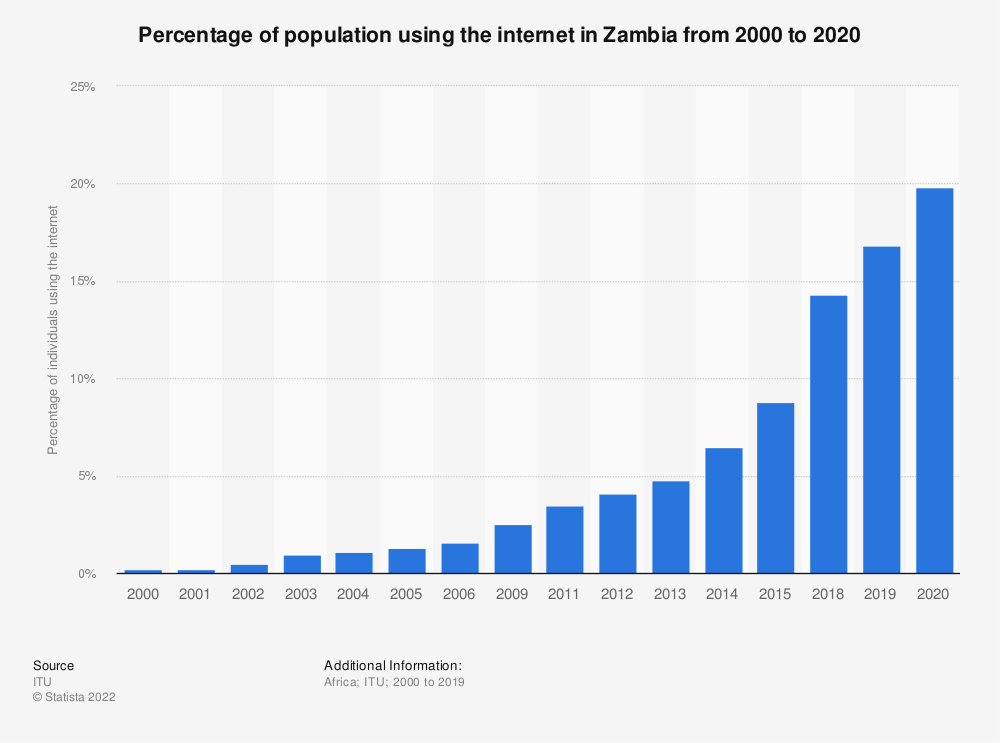
\includegraphics[width=6.25in,height=5.20833in]{Zambia_internet_penetration.png}

\begin{itemize}
\item
  As it is visible from the histogram around 2016 there has been a
  \textbf{significant increase in the internet acce}ss preceded by a
  steady increasing trend across all the previous years, and the
  literature reports this spike to be related mainly to a more diffused
  access to mobile internet. At the same time Zambia has hold two main
  elections in the period around the increase in the mobile connection
  bandwidth: one in 2011 and one in 2016.
\item
  Therefore, the aim of this project is to assess how the possibility to
  connect to the internet might affect socio-economic structures of
  political governance through channels such as: a change in social
  cohesion, an effect on democratic participation and open competition
  or also a change in the political game that reshuffle power dynamics
  across parties thanks to a change in instrument for political
  communication.
\end{itemize}

Many are the potential channels through which internet connection could
affect outcomes related to political governance and more broadly the
relationship of citizens with the state.

\begin{itemize}
\tightlist
\item
  The specific goal of the report is to \textbf{assess whether
  heterogeneity in mobile access connection is correlated with the
  presence of different levels of voters turnout, that is proxying
  electoral participation, or with different levels of valid votes,
  proxying a better understanding of the democratic competition rules}.
\end{itemize}

Three main datasets are used:

Firstly from the open election archives the shape of the electoral
district of Zambia is taken and putted together with data coming from
the OpenCellID website with an API to obtain the allocation of mobile
phone towers to the electoral districts.

Then always from the open election archives electoral district level
data on the electoral outcomes of the 2016 lower chamber election are
employed.

The the two following figures is visible how both voters turnout and the
number of mobile cells towers have a different geographical distribution
across districts:

\hypertarget{geographical-distribution-of-the-voters-turnout}{%
\subsubsection{Geographical Distribution of the voters'
turnout}\label{geographical-distribution-of-the-voters-turnout}}

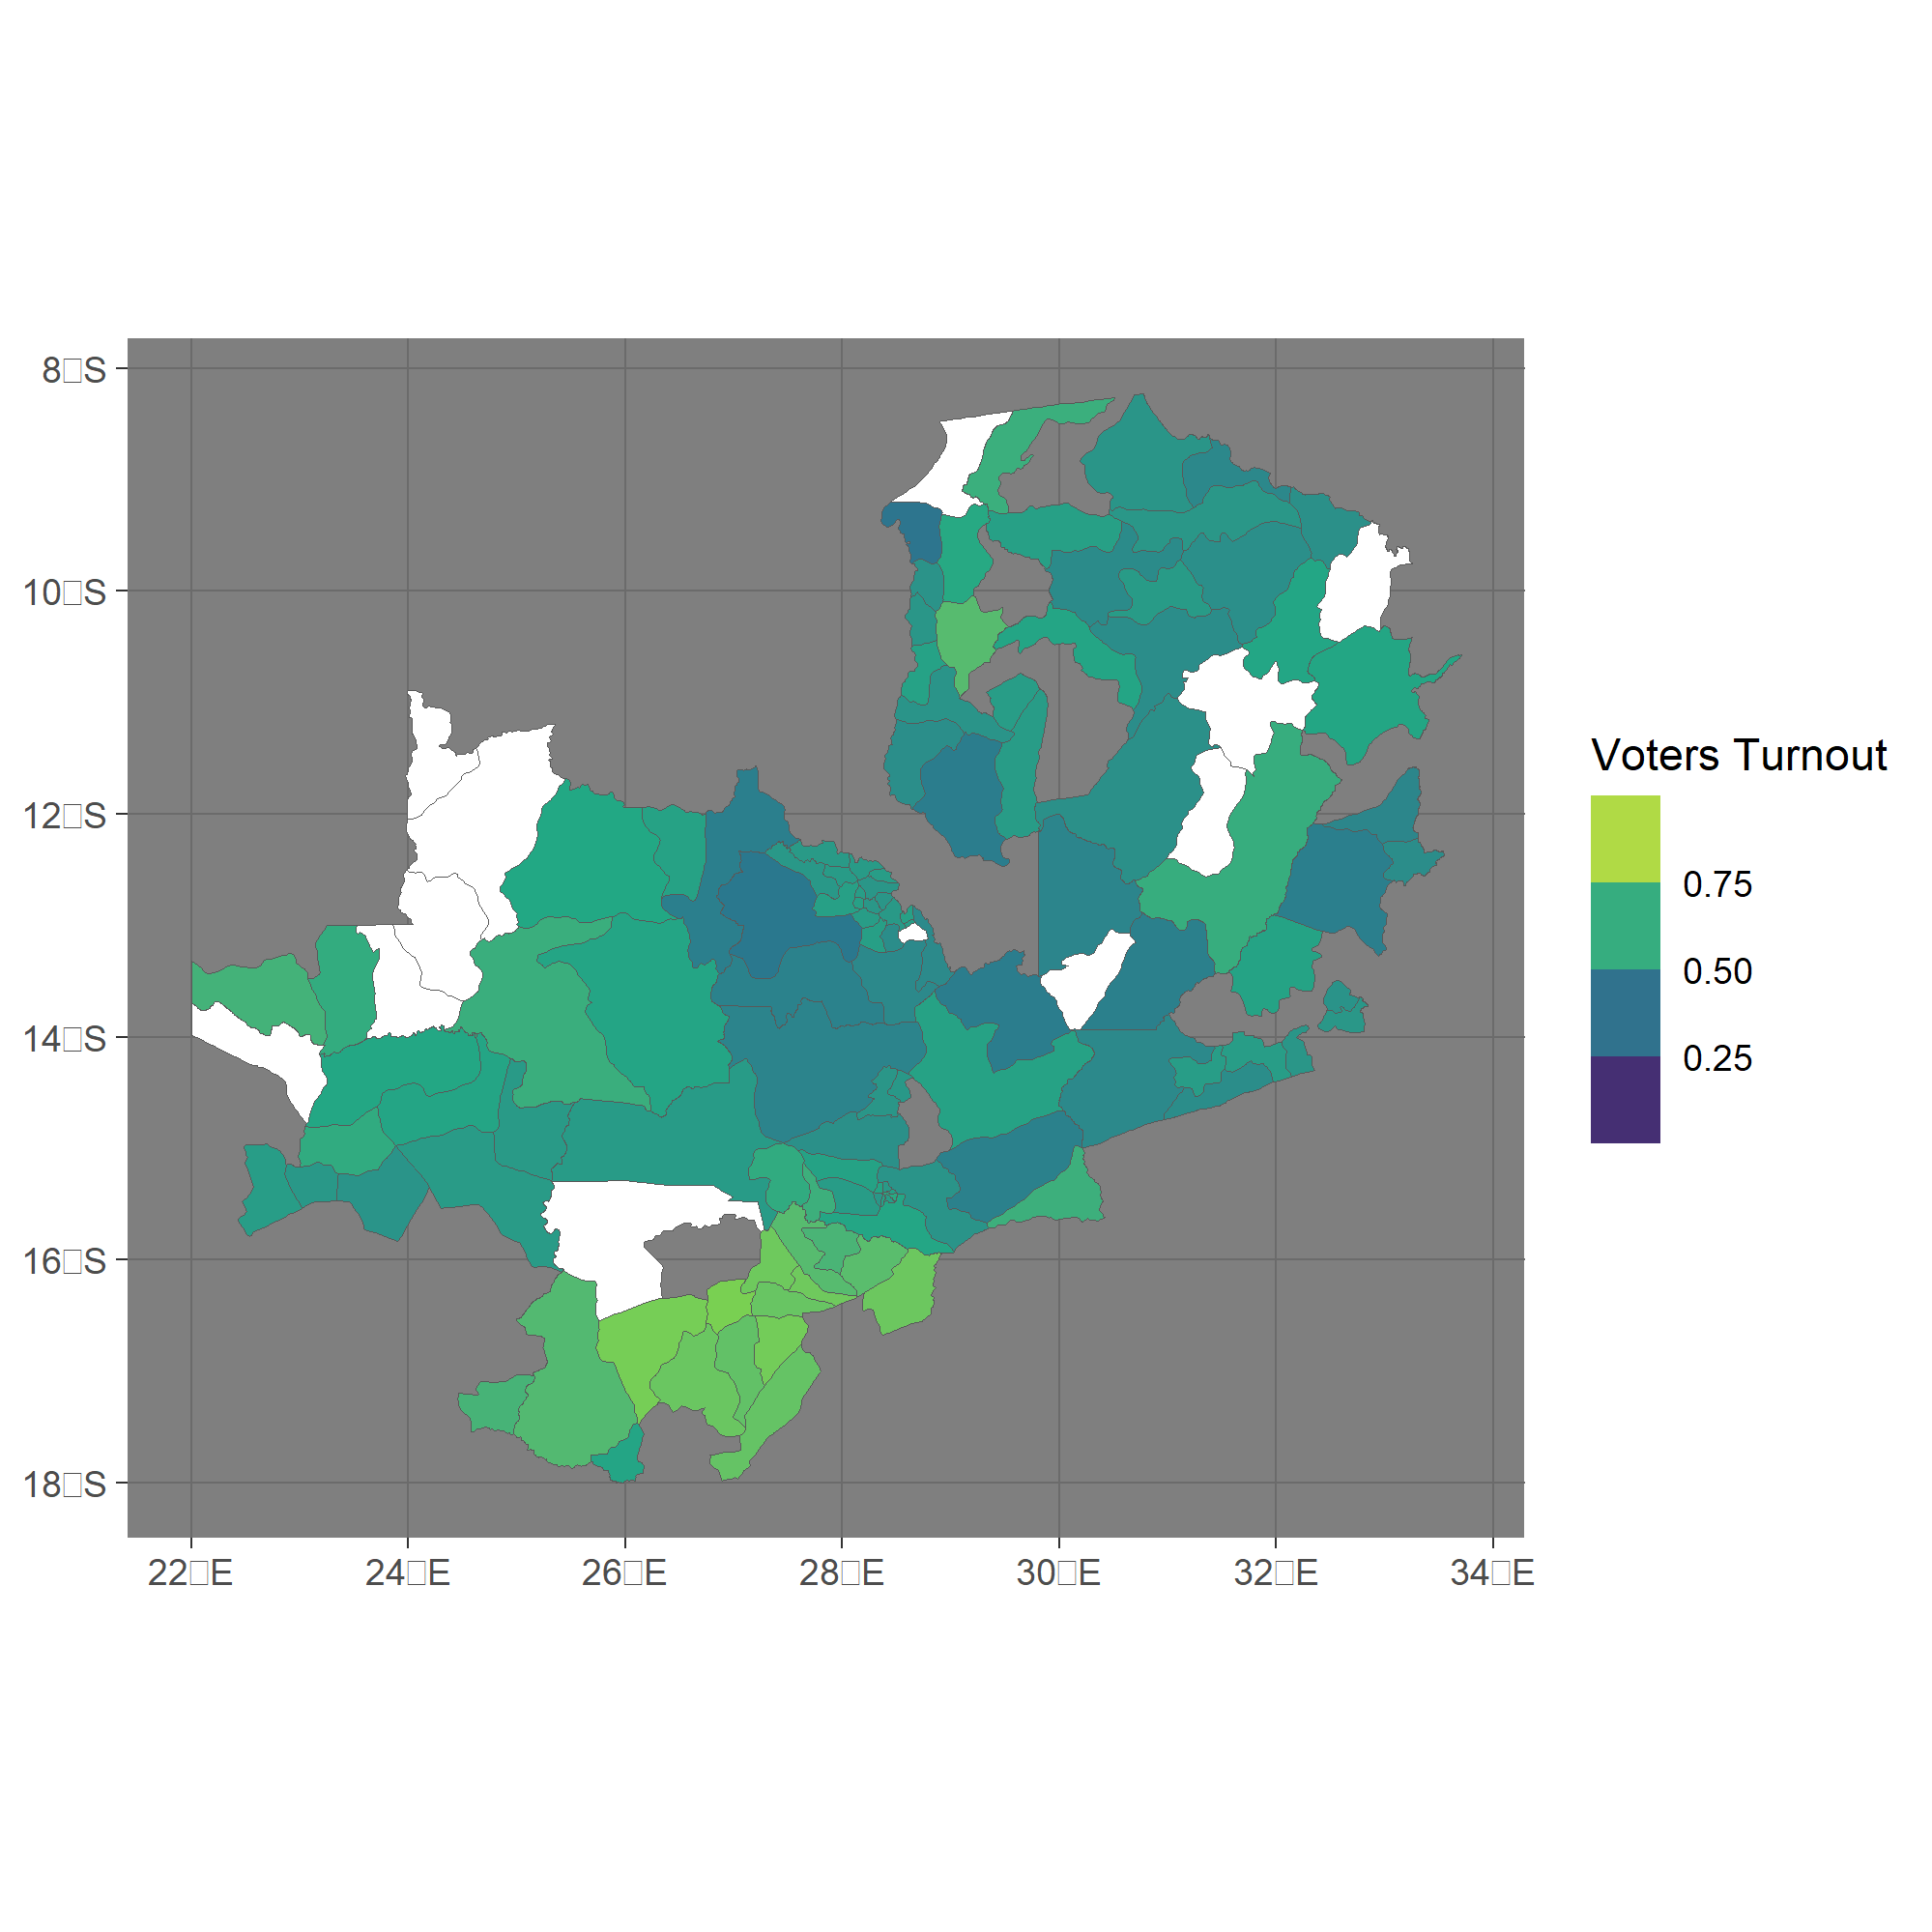
\includegraphics[width=3.125in,height=4.16667in]{outcome1.png}

\hypertarget{geographical-distribution-of-internet-mobile-cells}{%
\subsubsection{Geographical Distribution of internet mobile
cells}\label{geographical-distribution-of-internet-mobile-cells}}

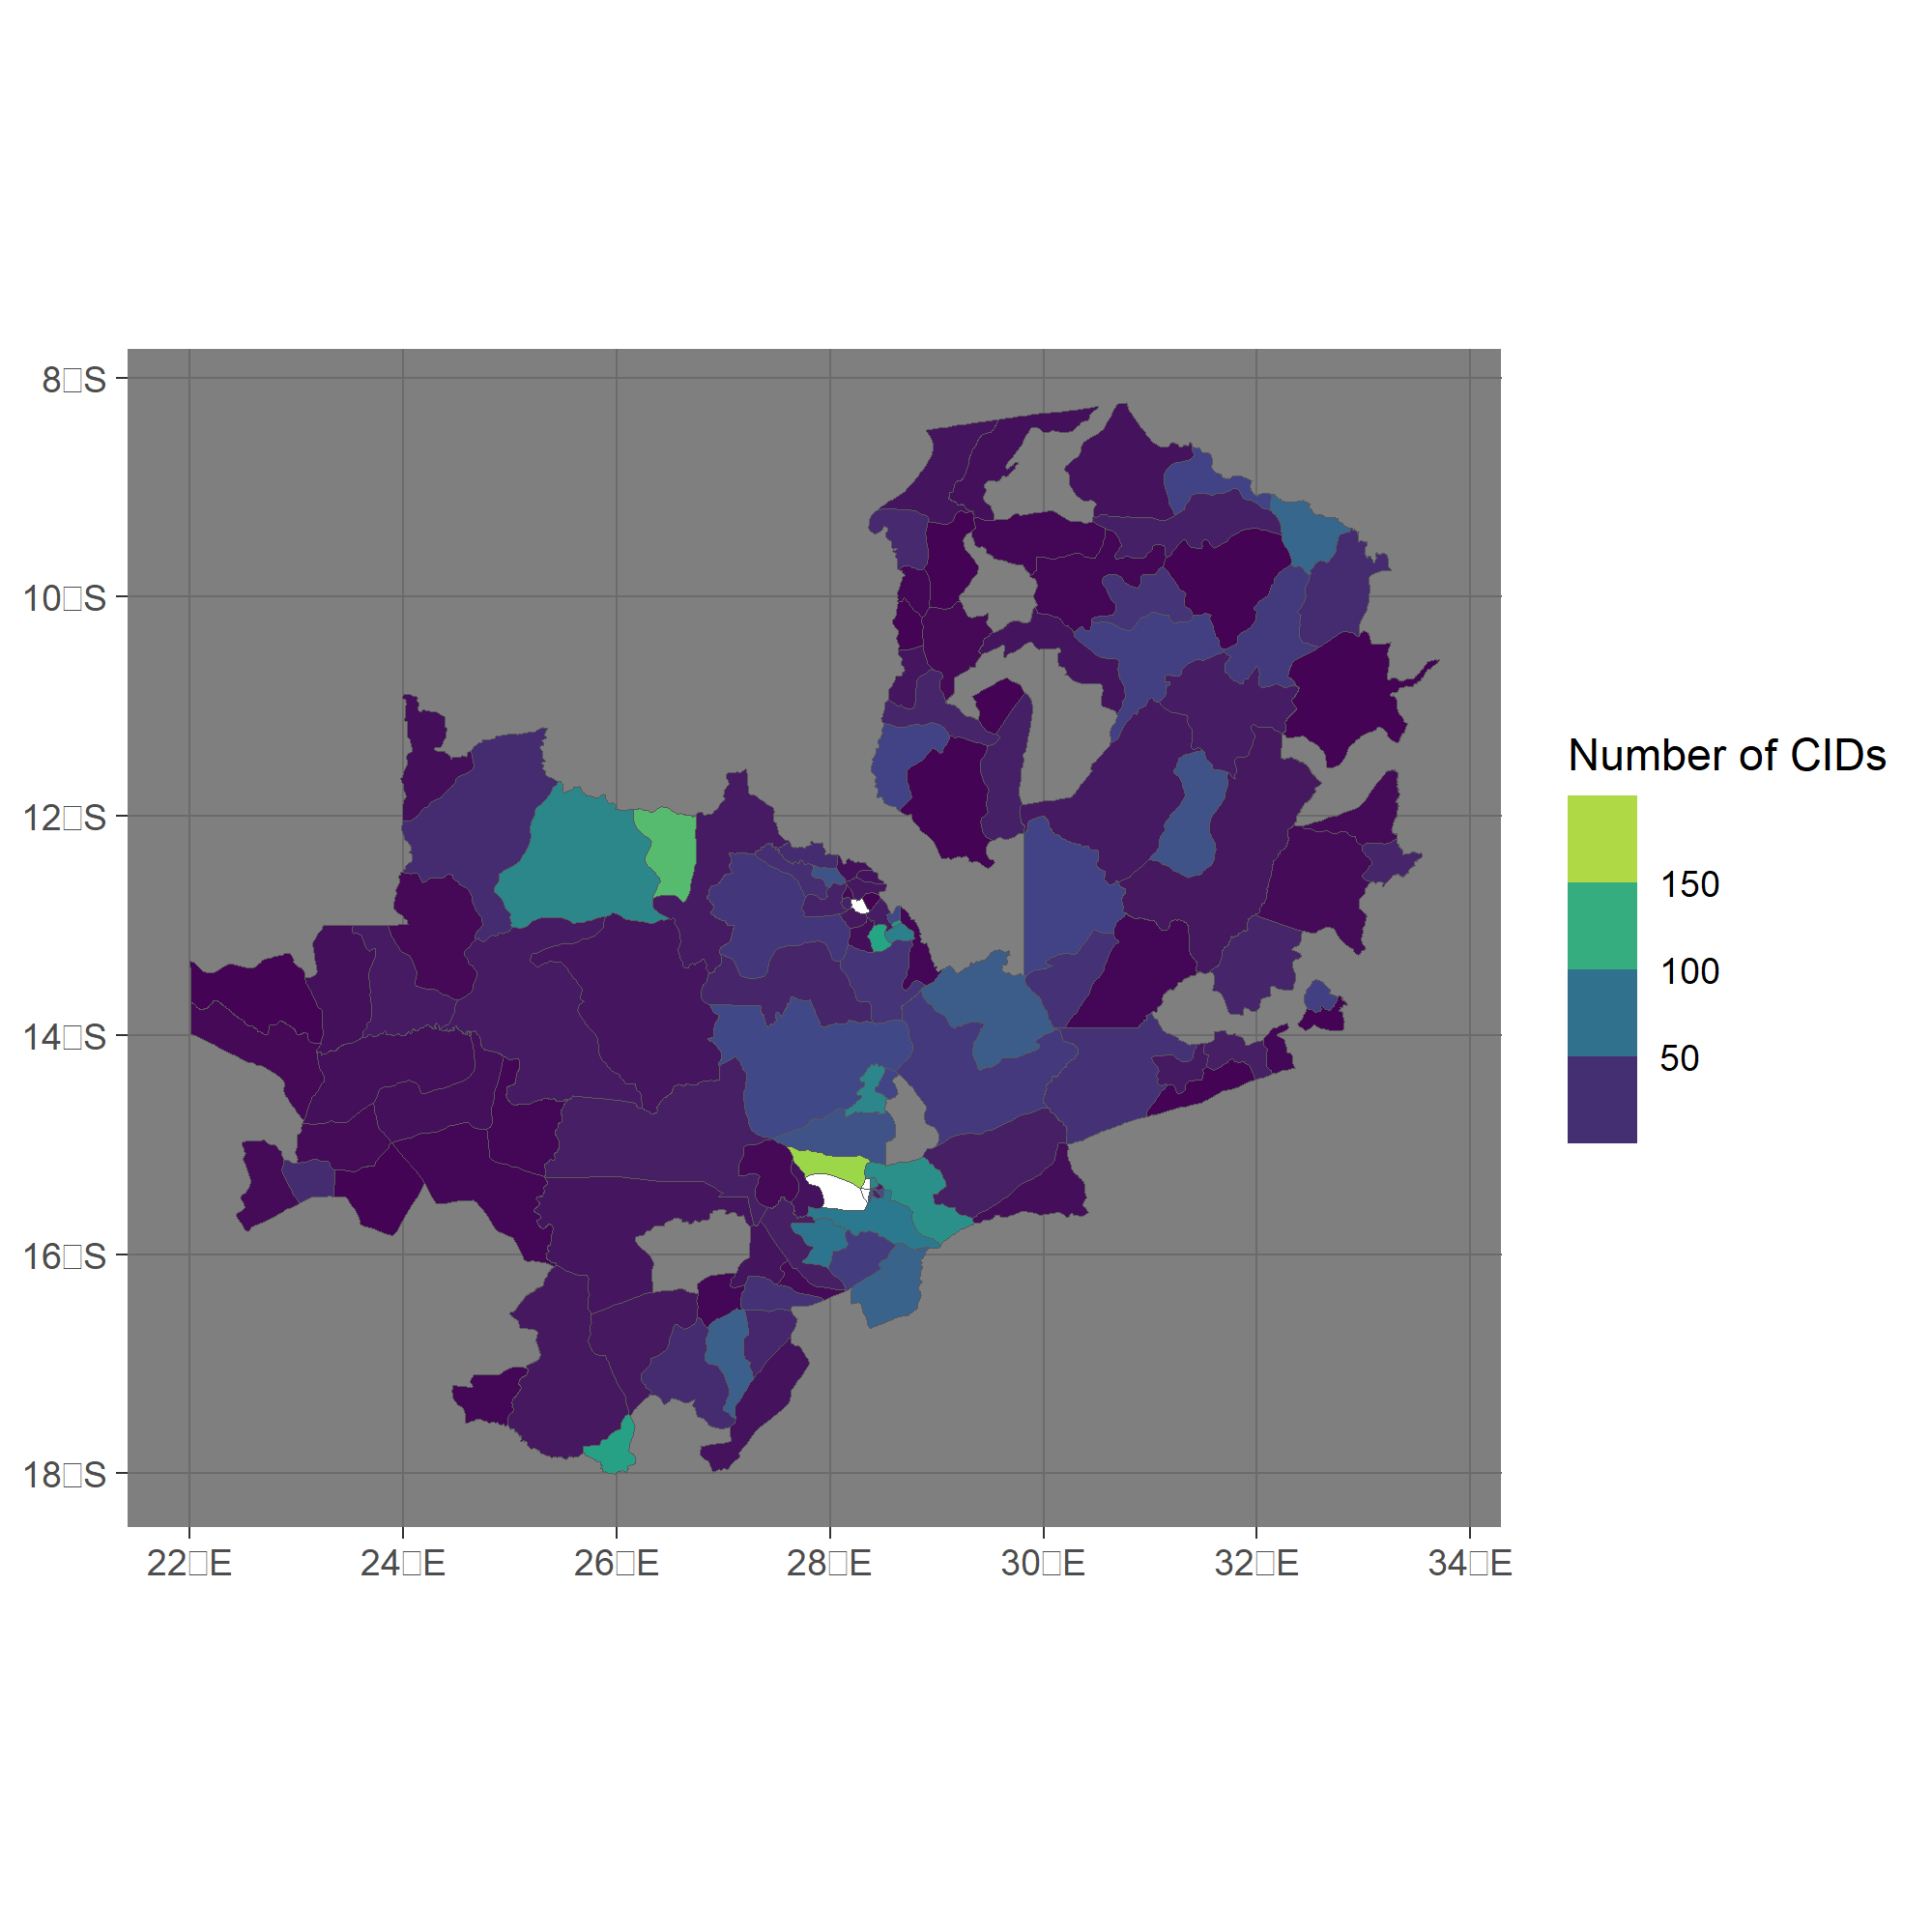
\includegraphics[width=3.125in,height=4.16667in]{treat1.png}

The research project finds that there is \textbf{little to no
correlation between both the electoral participation, the number of
eligible votes and the internet access} as visible in the correlation
plot below.

This could be happening because there is a lot of \textbf{measurement
error} in the mobile access given that the data are taken from an open
source system where users voluntarily register the presence of internet
cells.

Or alternatively it could e because there is already a minimum level of
internet everywhere by 2016 and therefore it is no more so crucial for
electoral outcomes.

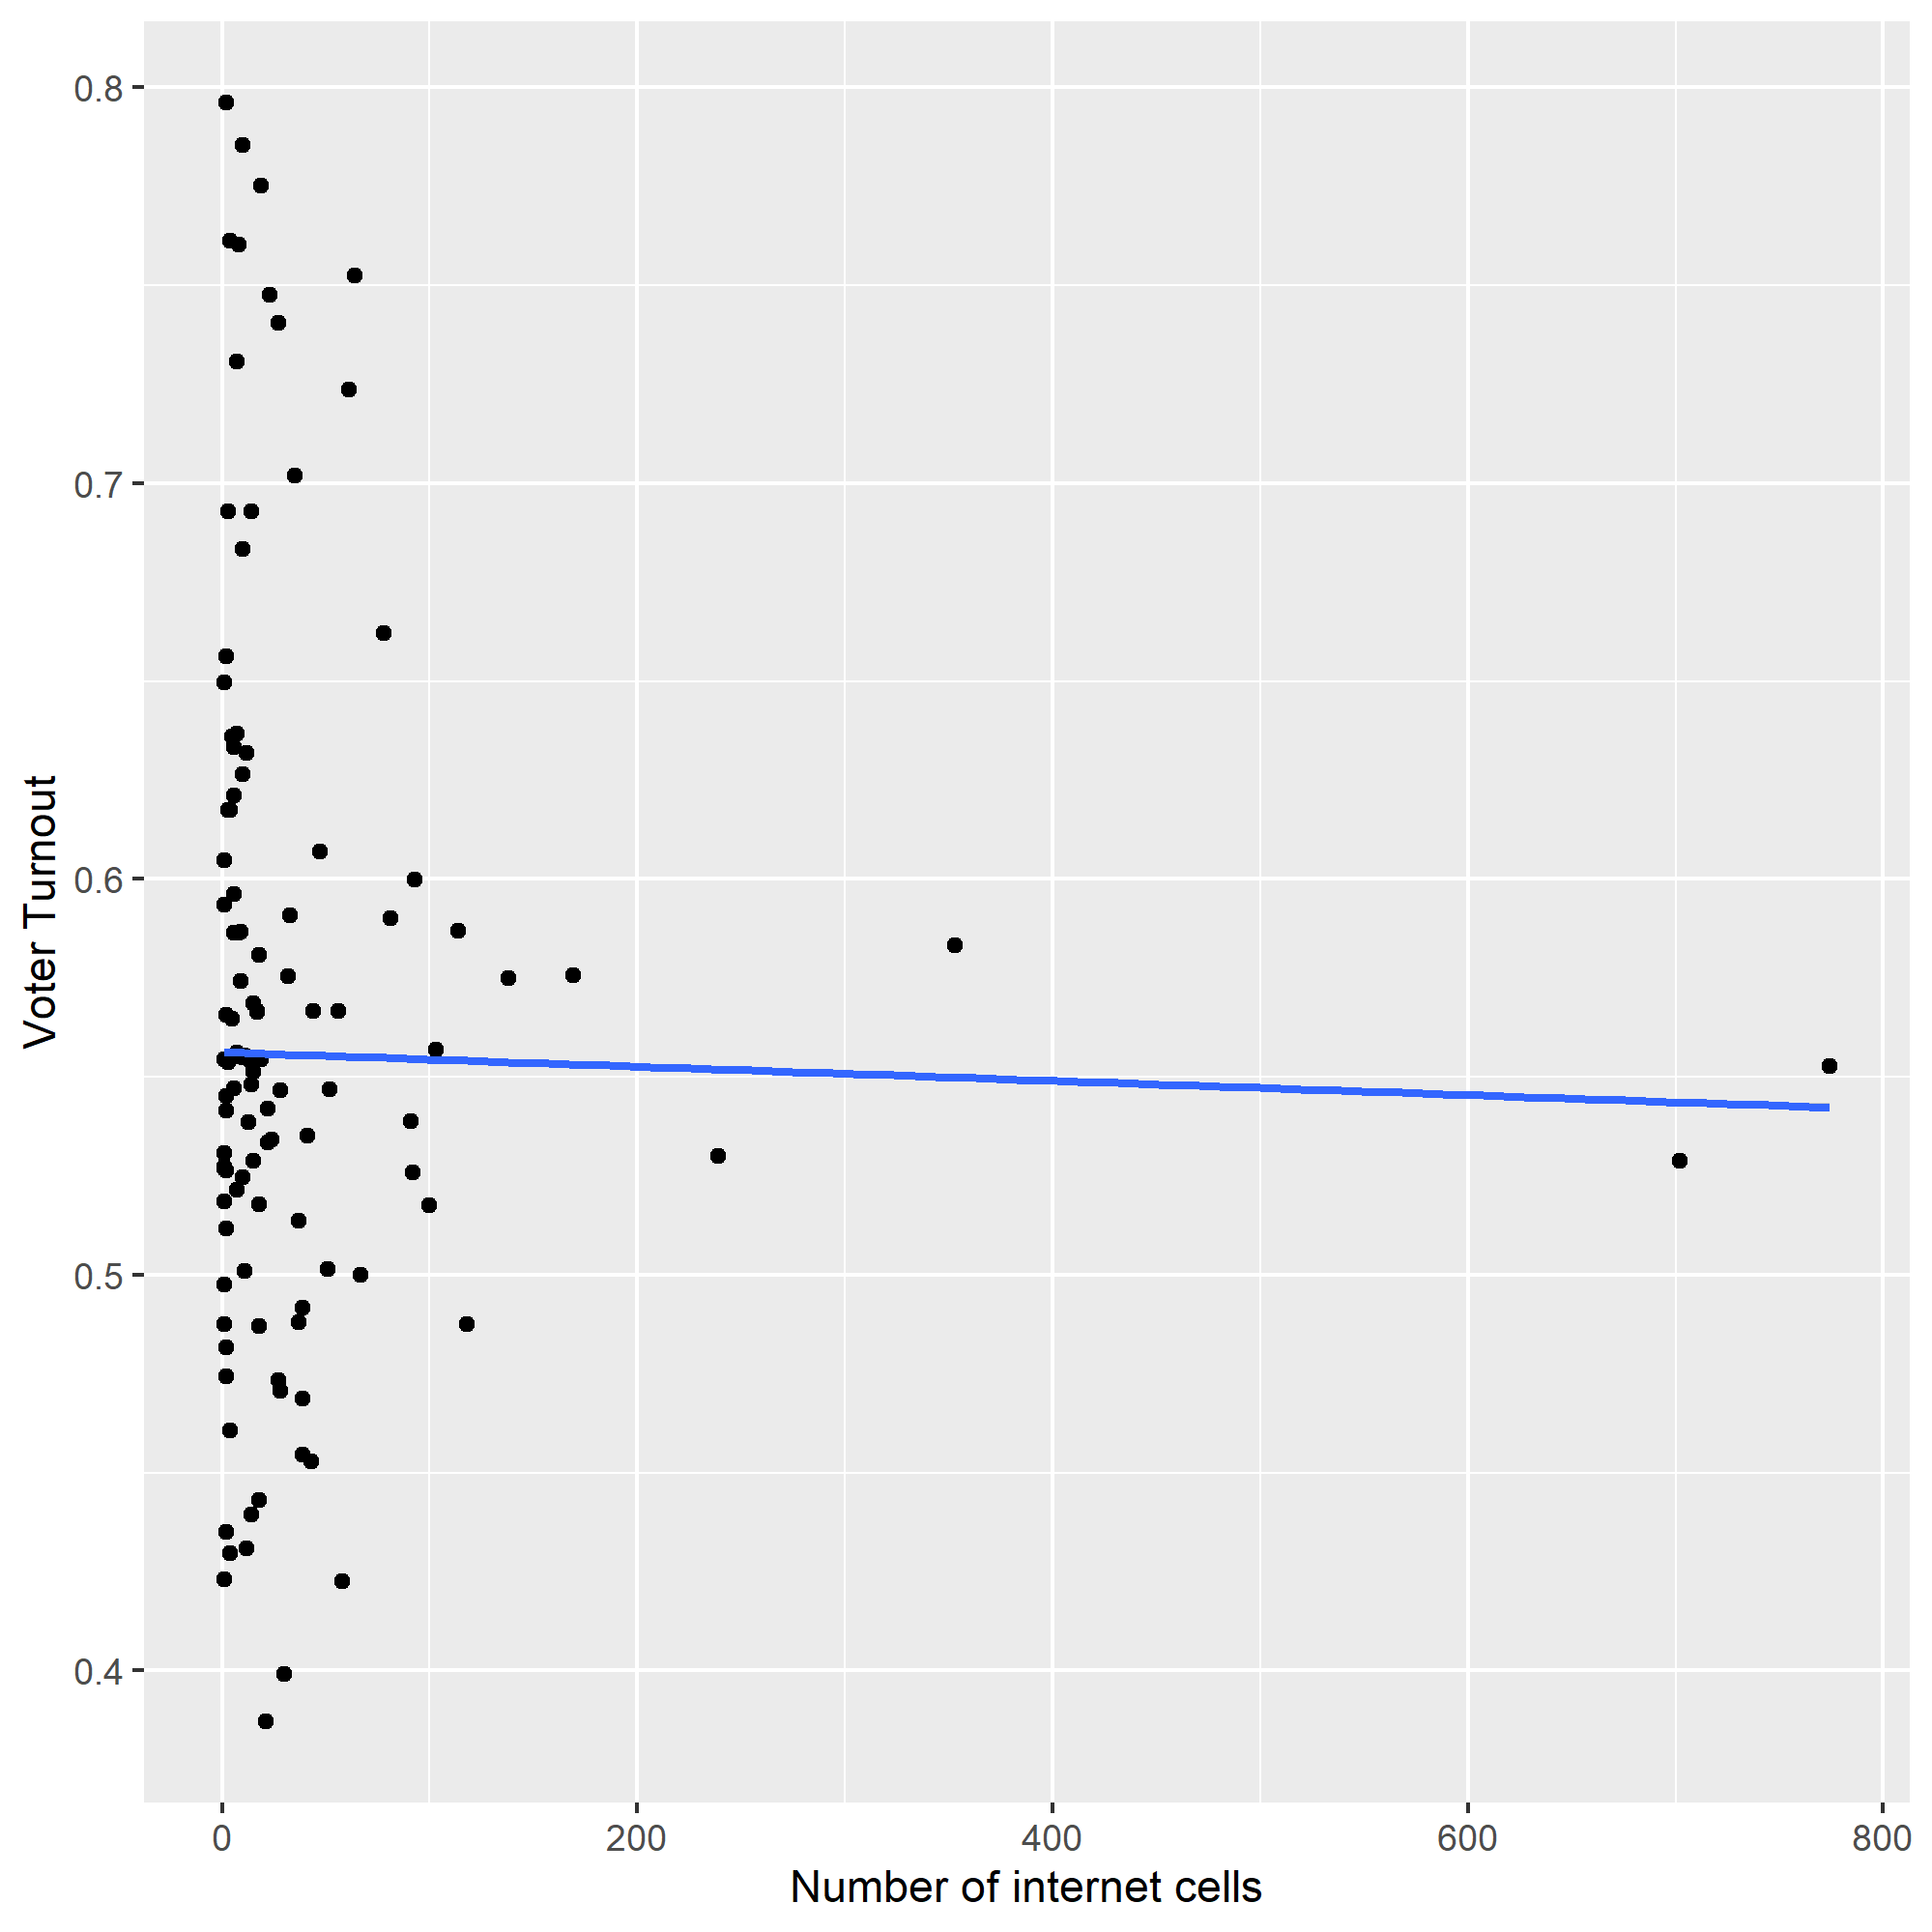
\includegraphics[width=6.25in,height=5.20833in]{lm.png}

The project also explores the patterns of partisan vote across
geographical units, finding a different geographical division for the
votes to the two main parties with NRP taking the majority of its votes
from the North-East and MMP winning across the South West.

\hypertarget{introduction}{%
\section{Introduction:}\label{introduction}}

The project employees 3 dataset with the aim to combine geo-referenced
election outcomes at electoral district level in Zambia with OpenCellID
data coming from a public access API containing information on the
presence of active internet cells and their coverage.

Firstly, I upload the data containing the geo-referenced information on
internet access downloaded from :
\url{https://opencellid.org/downloads.php} and I rename the columns so
that it is understandable which values is what and I keep only
interesting columns , to obtain the data as below as save them in a csv.

\begin{longtable}[t]{cccccc}
\caption{\label{tab:upload}\resizebox{\textwidth}{!}{Mobile access in Zambia raw data}}\\
\toprule
CID & Location\_Area\_Code & lat & lon & Range & Created\\
\midrule
62893 & 10004 & 28.27491 & -15.47154 & 2822 & 1459772900\\
2972 & 11108 & 28.33001 & -15.43928 & 6474 & 1459774040\\
62892 & 10004 & 28.28792 & -15.47047 & 1300 & 1459772900\\
33083 & 1 & 28.25304 & -15.46148 & 1000 & 1369370001\\
33081 & 1 & 28.25134 & -15.45296 & 1000 & 1369353306\\
\addlinespace
33933 & 1 & 28.24974 & -15.44518 & 1000 & 1369353496\\
\bottomrule
\end{longtable}

Then I transform the data from csv to a shape file creating a variable
called geometry containing the information now stored in the variables
latitude and longitude.

I keep only variables for which there are no missing data for longitude
and latitude, otherwise I do not know where to place them in the map and
I assign a coordinate reference system so that I can compare this map
with the map that I will use later containing the data on the elections,
to obtain the shape file of the mobile data as below:

The data on mobile access are now in shape-file format and look like
this :

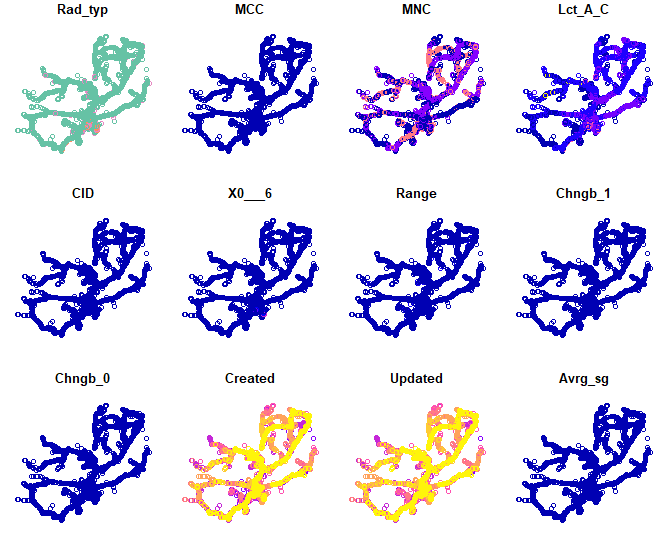
\includegraphics[width=3.125in,height=4.16667in]{mobile_access_new.png}

Here we can already see the shape of Zambia even if the borders are not
clear, we see how the different variables in the dataset are distributed
across the coordinates of Zambia. For now this is not particularly
indicative of anything, beside that the internet access data have been
successfully converted into a shape-file.

Now to give Zambia a shape and to upload the remaining part of the data
necessary for the analysis I open from
\url{https://electiondataarchive.org/data-and-documentation/georeferenced-electoral-districts-datasets/}
the shapes of the Zambian electoral districts, I assign the same
coordinate reference system that I assigned to the mobile data above and
I obtain the data as below:

\begin{verbatim}
## Reading layer `gred' from data source `/home/marta/Zambia/gred.shp' using driver `ESRI Shapefile'
## Simple feature collection with 150 features and 5 fields
## Geometry type: POLYGON
## Dimension:     XY
## Bounding box:  xmin: 21.99937 ymin: -18.07947 xmax: 33.7057 ymax: -8.22436
## CRS:           NA
\end{verbatim}

\begin{longtable}[t]{cccccc}
\caption{\label{tab:newshape}\resizebox{\textwidth}{!} {Shape of electoral districts in Zambia}}\\
\toprule
ctr\_n & ctr & yr & cst\_n & cst & geometry\\
\midrule
Zambia & 894 & 2006 & Mfuwe & 94 & POLYGON ((32.23695 -11.2491...\\
Zambia & 894 & 2006 & Kawambwa & 61 & POLYGON ((29.34078 -9.27867...\\
Zambia & 894 & 2006 & Nyimba & 128 & POLYGON ((31.42754 -14.0779...\\
Zambia & 894 & 2006 & Solwezi West & 146 & POLYGON ((26.15134 -11.9382...\\
Zambia & 894 & 2006 & Kapiri Mposhi & 53 & POLYGON ((28.38889 -13.8794...\\
\addlinespace
Zambia & 894 & 2006 & Lufwanyama & 72 & POLYGON ((27.28778 -12.3438...\\
\bottomrule
\end{longtable}

Plotting the data we can see how they report the coordinates of each
electoral district in Zambia:

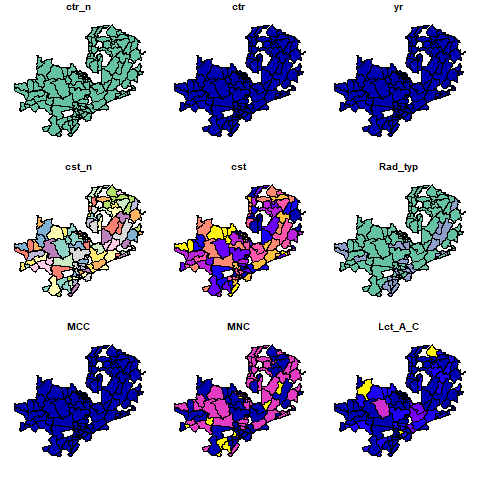
\includegraphics[width=3.125in,height=\textheight]{gred.png}

\hypertarget{data-exploration}{%
\section{Data exploration}\label{data-exploration}}

Now that I have both the mobile phone information and the shape of the
electoral districts I can start exploring the variables of interest to
answer to my research questions:

\hypertarget{which-is-the-effect-of-internet-access-measured-as-the-presence-of-an-active-registered-cid-in-the-electoral-district-on-electoral-outcome-partisan-vote-and-number-of-valid-votes}{%
\subsection{1) Which is the effect of internet access, measured as the
presence of an active registered CID in the electoral district, on
electoral outcome, partisan vote and number of valid
votes?}\label{which-is-the-effect-of-internet-access-measured-as-the-presence-of-an-active-registered-cid-in-the-electoral-district-on-electoral-outcome-partisan-vote-and-number-of-valid-votes}}

\hypertarget{how-the-results-change-when-the-presence-of-internet-access-is-measured-using-the-fact-that-there-is-at-least-one-cell-in-the-district}{%
\subsection{2) How the results change when the presence of internet
access is measured using the fact that there is at least one cell in the
district
?}\label{how-the-results-change-when-the-presence-of-internet-access-is-measured-using-the-fact-that-there-is-at-least-one-cell-in-the-district}}

I start by looking at how the presence of internet cells are distributed
in the geography looking at all the data available regardless of the
year:

\hypertarget{presence-if-internet-cells}{%
\paragraph{Presence if Internet
Cells}\label{presence-if-internet-cells}}

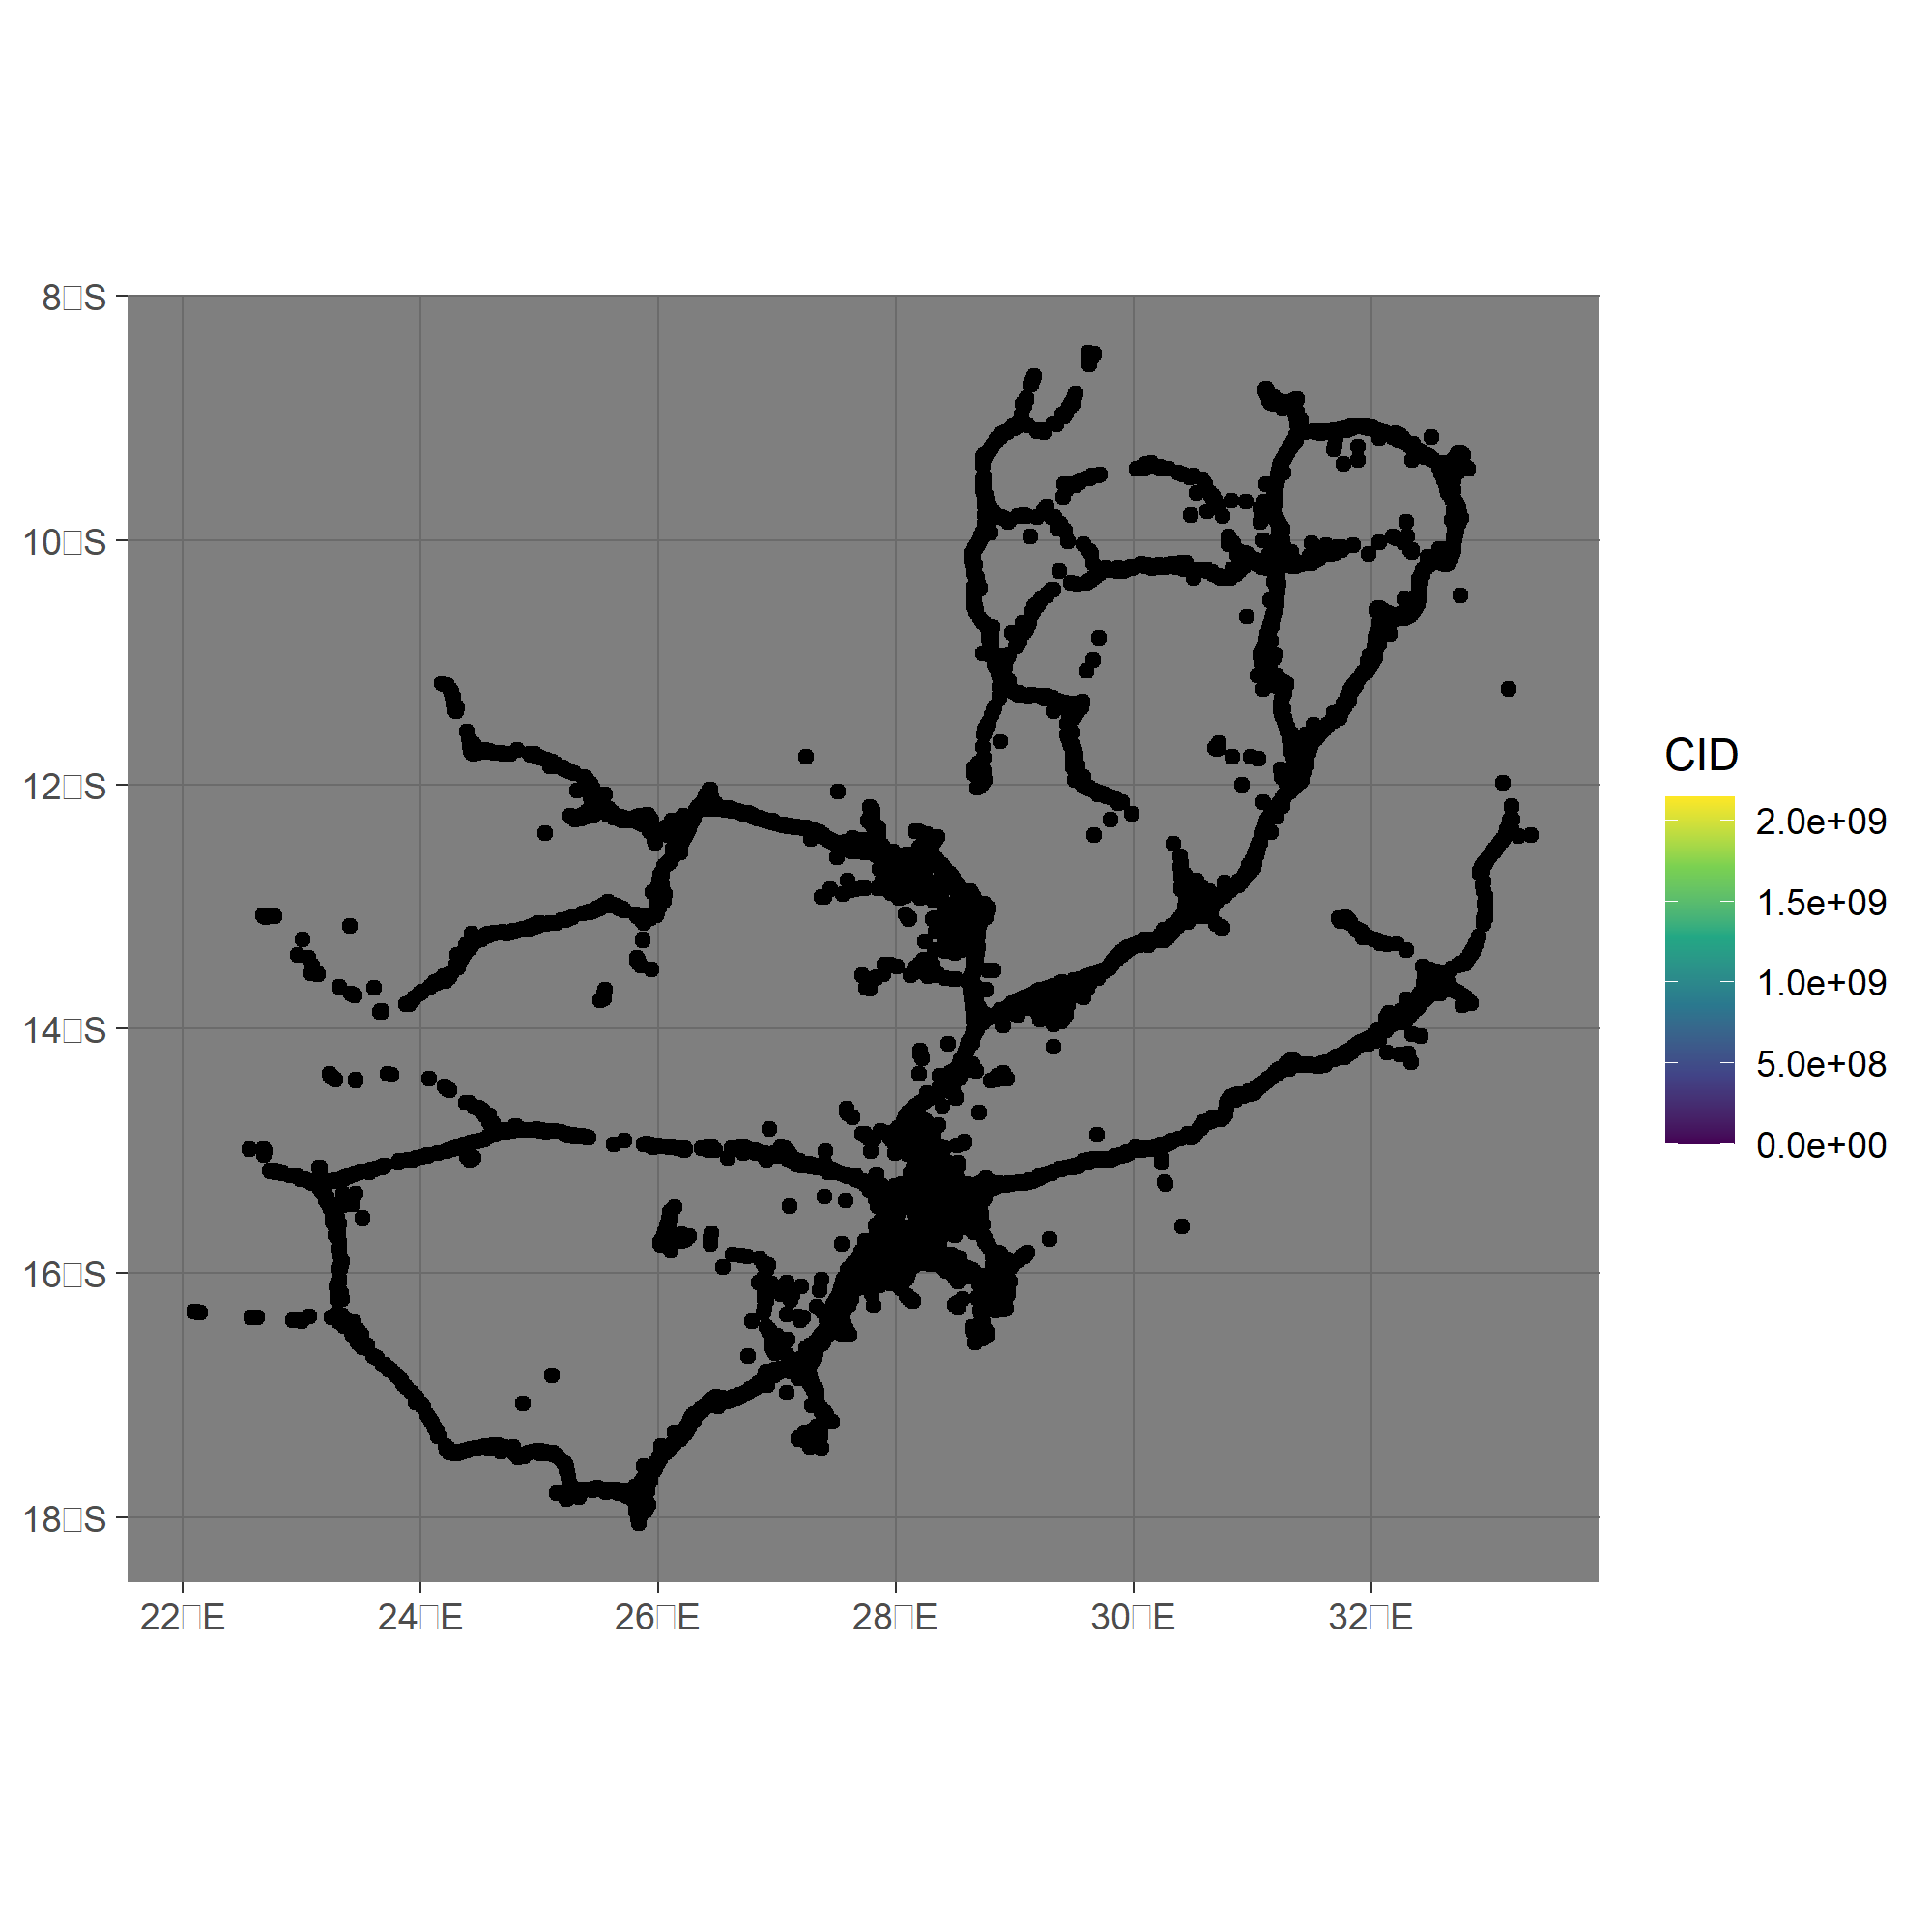
\includegraphics[width=4.16667in,height=3.125in]{presence_cells.png}

It is visible how considering all the years at the same time there are
CID bringing internet all across the country.

Now to consider only data for the years of interest for the elections I
slice the dataset into years using the column called created.

To do so I first convert the timestamp into a date, it is a Unix
timestamp so it is indicating the number of seconds from a fixed date
and is unreadable as it is.

The I create a list of years and I loop through it to create one dataset
for each year. I'm interested in years 2011 and 2016 that can be seen
below:

\hypertarget{section}{%
\subsection{2011}\label{section}}

\begin{longtable}[t]{cccccccccccccc}
\caption{\label{tab:anotheryear}\resizebox{\textwidth}{!} {Mobile access in 2011}}\\
\toprule
Radio\_type & MCC & MNC & Location\_Area\_Code & CID & 0 & lat & lon & Range & Changeable=1 & Changeable=0 & Created & Updated & Average\_signal\\
\midrule
UMTS & 645 & 2 & 115 & 95744 & 0 & 32.76329 & -9.330826 & 1000 & 3 & 1 & 2011-05-07 11:45:38 & 1305121951 & 0\\
UMTS & 645 & 1 & 1008 & 103838 & 0 & 28.35777 & -15.371933 & 1000 & 1 & 1 & 2011-06-07 13:18:51 & 1307452731 & 0\\
\bottomrule
\end{longtable}

\hypertarget{section-1}{%
\subsection{2016}\label{section-1}}

\begin{longtable}[t]{cccccccccccccc}
\caption{\label{tab:year}\resizebox{\textwidth}{!} {Mobile access in 2016}}\\
\toprule
Radio\_type & MCC & MNC & Location\_Area\_Code & CID & 0 & lat & lon & Range & Changeable=1 & Changeable=0 & Created & Updated & Average\_signal\\
\midrule
GSM & 645 & 3 & 10004 & 62893 & 0 & 28.27491 & -15.471539 & 2822 & 62 & 1 & 2016-04-04 12:28:20 & 1563083742 & 0\\
GSM & 645 & 2 & 11108 & 2972 & 0 & 28.33001 & -15.439281 & 6474 & 139 & 1 & 2016-04-04 12:47:20 & 1601638171 & 0\\
GSM & 645 & 3 & 10004 & 62892 & 0 & 28.28792 & -15.470468 & 1300 & 62 & 1 & 2016-04-04 12:28:20 & 1564057707 & 0\\
GSM & 645 & 2 & 20003 & 551 & 0 & 26.24292 & -17.274475 & 22839 & 15 & 1 & 2016-04-03 15:59:42 & 1679970244 & 0\\
GSM & 645 & 1 & 10119 & 31421 & 0 & 31.31668 & -9.239495 & 13483 & 3 & 1 & 2016-04-04 11:10:12 & 1503554998 & 0\\
\addlinespace
UMTS & 645 & 1 & 1008 & 95990 & 0 & 28.29826 & -15.435104 & 1000 & 3 & 1 & 2016-03-24 23:13:55 & 1486432897 & 0\\
\bottomrule
\end{longtable}

As it is visible the data for 2011 contain only 2 observations so the
rest of the analysis will be focused on the 2016 elections.

I now open the mobile data for 2016 as a sf object (a way to call the
shape files when openend with specific libraries in R) and I assign
again always the same coordinate reference system.

Then I check and compare the coordinate reference system and make sure
they match.

At this point I can merge the file with the shape of the electoral
districts with the one of the mobile access in the year of interest for
which the data are available and then write the merged dataset into a
shapefile, so that I can see how many cells were in each district.

And the data look as below:

\begin{verbatim}
## Reading layer `y2016' from data source `/home/marta/Zambia/y2016.shp' using driver `ESRI Shapefile'
## Simple feature collection with 5498 features and 12 fields
## Geometry type: POINT
## Dimension:     XY
## Bounding box:  xmin: 22.67231 ymin: -17.92831 xmax: 33.34831 ymax: -8.46428
## Geodetic CRS:  WGS 84
\end{verbatim}

\begin{longtable}[t]{lcccccccccccccccccc}
\caption{\label{tab:merge}\resizebox{\textwidth}{!} {Election data into discrits' shapes}}\\
\toprule
  & ctr\_n & ctr & yr & cst\_n & cst & Rad\_typ & MCC & MNC & Lct\_A\_C & CID & X0 & Range & Chngb.1 & Chngb.0 & Created & Updated & Avrg\_sg & geometry\\
\midrule
1 & Zambia & 894 & 2006 & Mfuwe & 94 & GSM & 645 & 1 & 10115 & 30982 & 0 & 7830 & 16 & 1 & 2016-01-16 & 1565600127 & 0 & POLYGON ((32.23695 -11.2491...\\
1.1 & Zambia & 894 & 2006 & Mfuwe & 94 & GSM & 645 & 2 & 520 & 6242 & 0 & 6217 & 3 & 1 & 2016-02-24 & 1507040057 & 0 & POLYGON ((32.23695 -11.2491...\\
1.2 & Zambia & 894 & 2006 & Mfuwe & 94 & UMTS & 645 & 1 & 4108 & 232851 & 0 & 1000 & 1 & 1 & 2016-01-29 & 1454053584 & 0 & POLYGON ((32.23695 -11.2491...\\
1.3 & Zambia & 894 & 2006 & Mfuwe & 94 & UMTS & 645 & 1 & 4108 & 231551 & 0 & 1672 & 3 & 1 & 2016-03-24 & 1481287116 & 0 & POLYGON ((32.23695 -11.2491...\\
1.4 & Zambia & 894 & 2006 & Mfuwe & 94 & GSM & 645 & 1 & 10115 & 35262 & 0 & 14698 & 12 & 1 & 2016-07-03 & 1574074515 & 0 & POLYGON ((32.23695 -11.2491...\\
\addlinespace
1.5 & Zambia & 894 & 2006 & Mfuwe & 94 & GSM & 645 & 1 & 465 & 4051 & 0 & 3748 & 7 & 1 & 2016-03-25 & 1523586610 & 0 & POLYGON ((32.23695 -11.2491...\\
\bottomrule
\end{longtable}


\includegraphics[width=6.25in,height=5.20833in]{thejoin.png}

Now I can rename variables knowing that :

CID = number of mobile cells

Geometry = location

Range = range of functioning of the tower

\hypertarget{statistical-analysis}{%
\section{Statistical Analysis}\label{statistical-analysis}}

\hypertarget{first-treatment-assignation}{%
\subsubsection{First treatment
assignation}\label{first-treatment-assignation}}

I can now start to see how the number of a CID mobile internet cells is
correlated with district level electoral outcomes from the lower chamber
election in 2016. To do this I start by creating a new variables that is
corresponding to the amount of internet mobile cells present in the
electoral district, this is going to be the non-experimental treatment
that I will try to leverage on in the analysis. After creating the new
variable I plot it's geographical distribution using a white patch for
variables with no data (NA):

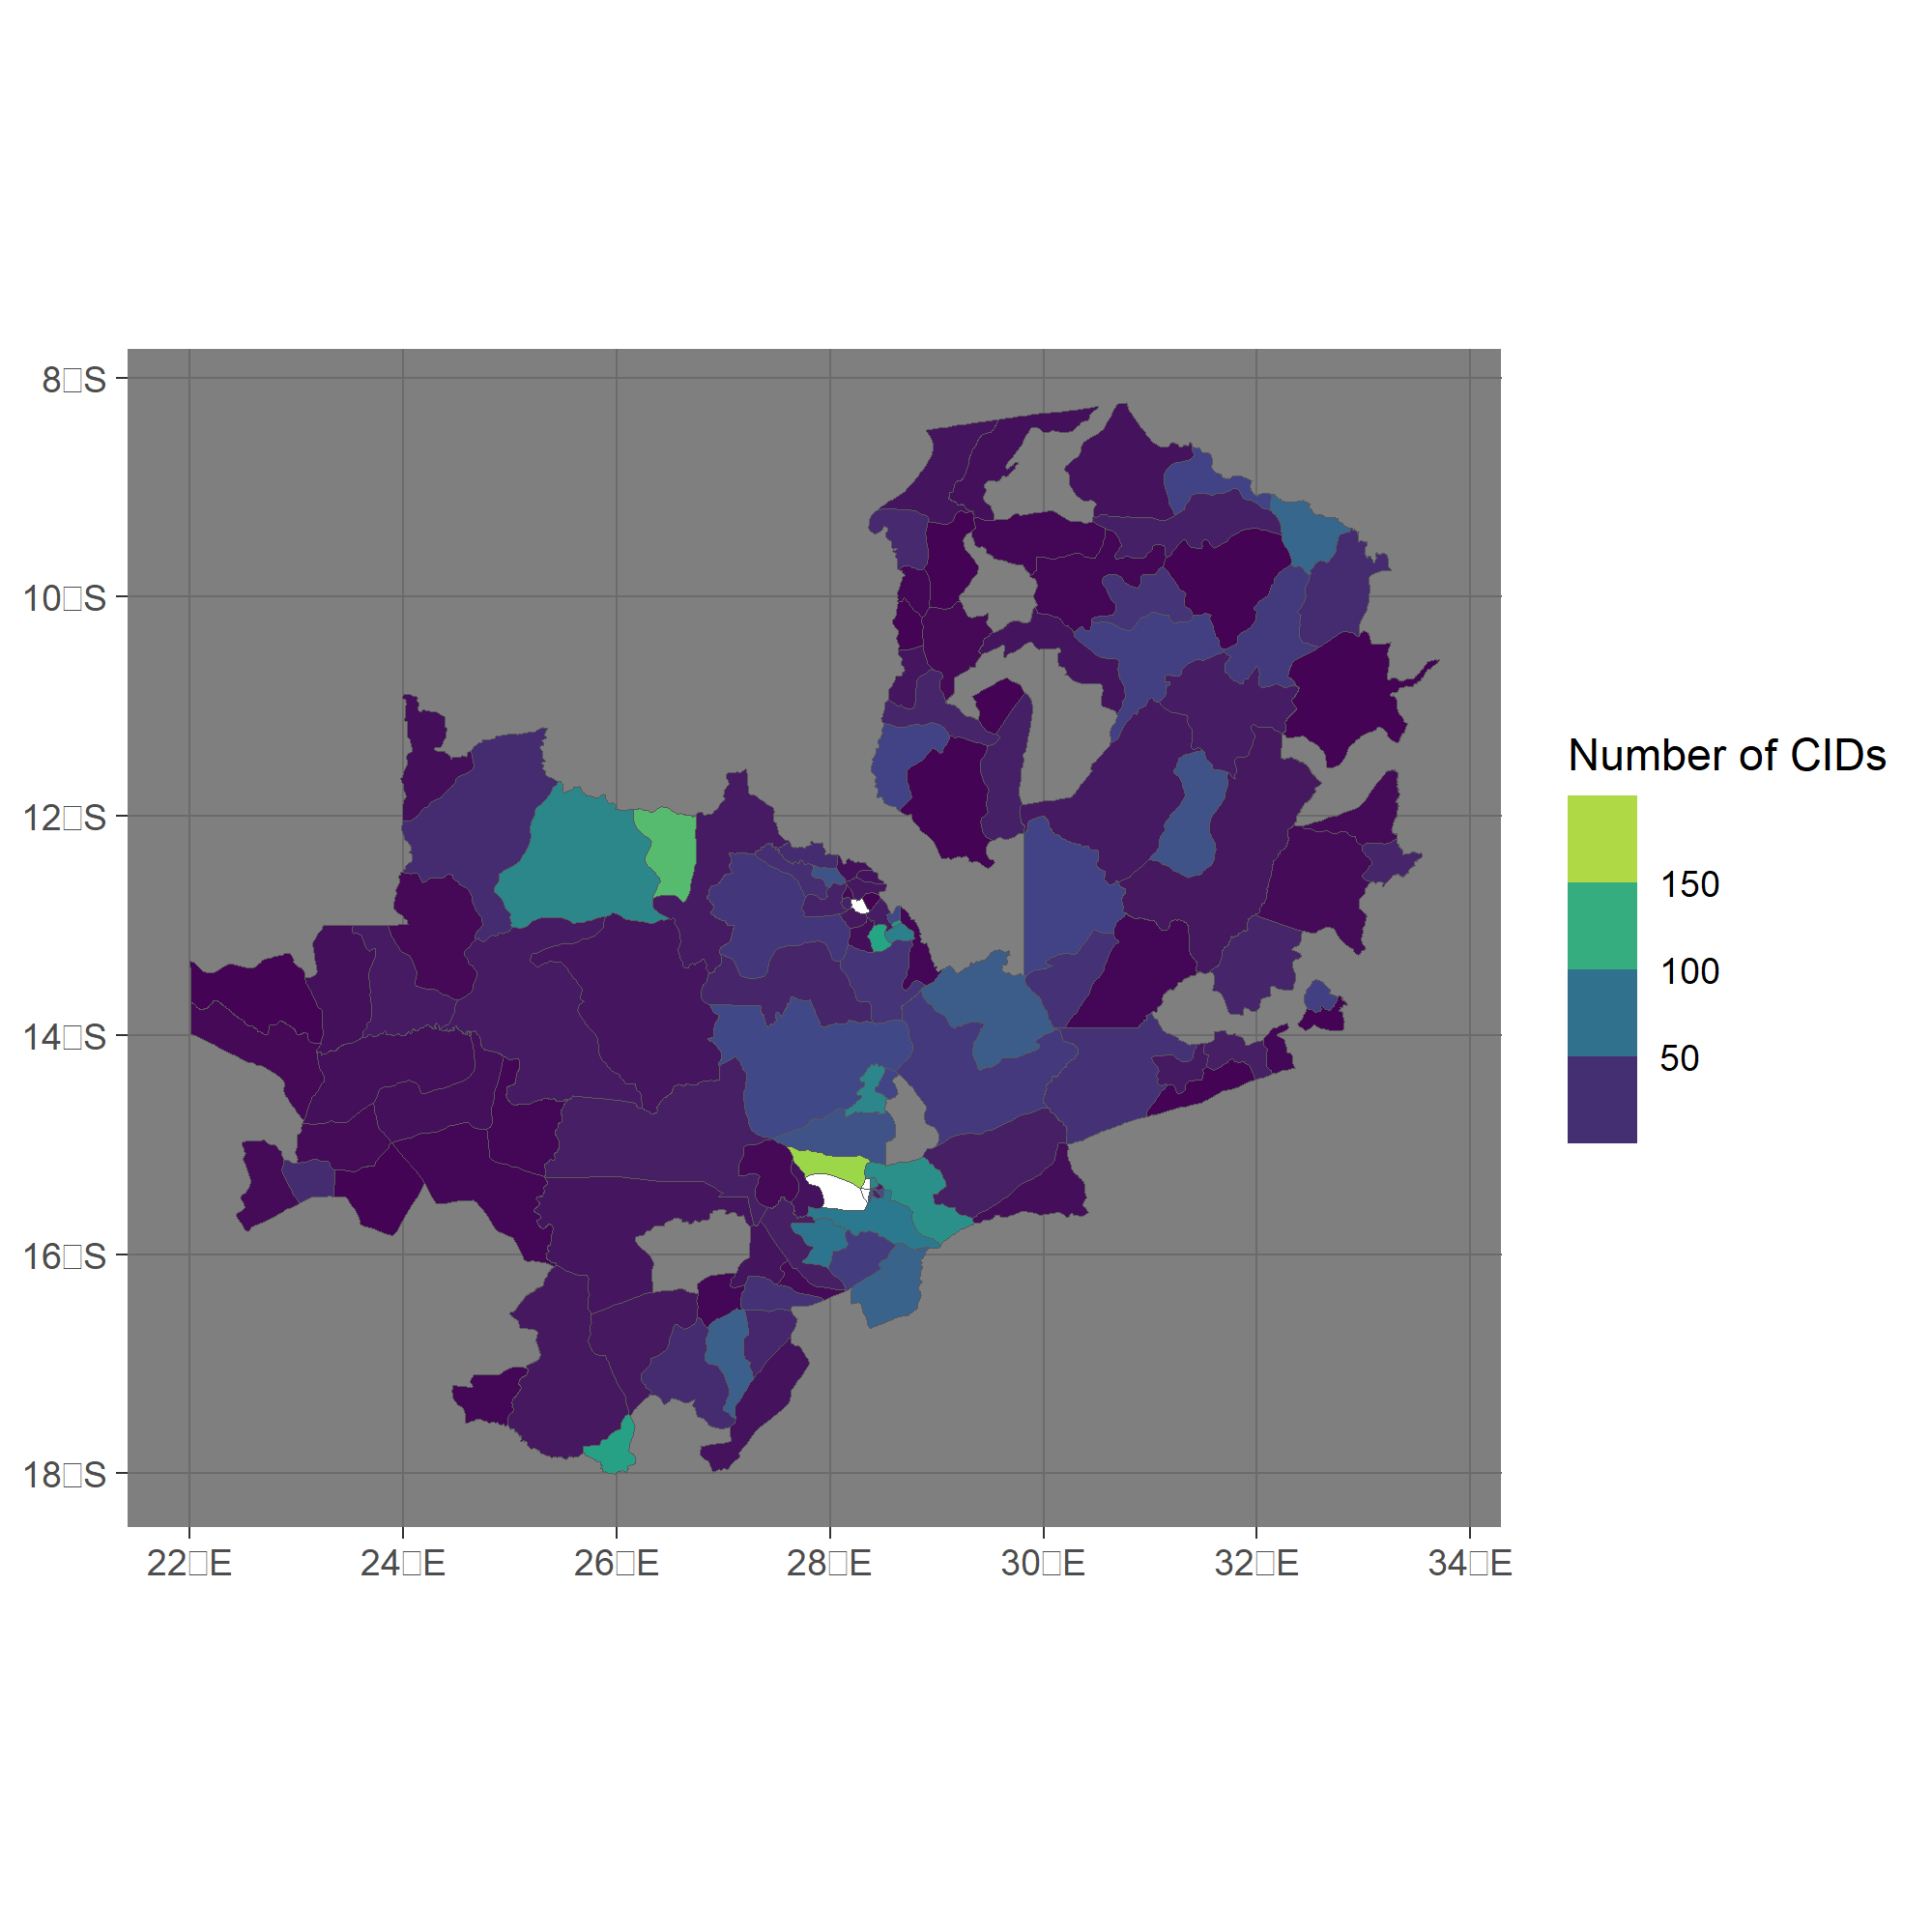
\includegraphics[width=6.25in,height=5.20833in]{treat1.png}

Looking at the map above the lighter is the color the higher is the
number of mobile cells and the picture suggests that there is
heterogeneity in the intensity of the internet across different
electoral districts.

At this point I can upload the data on the election for Zambia in 2016
taking them from
\url{https://electiondataarchive.org/data-and-documentation/clea-lower-chamber-elections-archive/}
to see how it correlates with this first treatment assignation.

The data on the elections need to be cleaned, so I keep only useful
column and then rename them to obtain the dataset below:

\begin{longtable}[t]{ccccccccccc}
\caption{\label{tab:clean}\resizebox{\textwidth}{!} {Lower Chamber 2016 election data}}\\
\toprule
elec\_district\_name & party\_name & party\_code & n\_eligible\_voters & n\_valid\_votes & voter\_turn & cvs1 & n\_votes & party\_vpte\_share & vote\_cast & n\_invalid\_votes\\
\midrule
BAHATI & Patriotic Front & 23 & 43827 & 22222 & 0.5177858 & 0.8174782 & 18166 & 0.8174782 & 22693 & 471\\
BAHATI & United Party for National Development & 29 & 43827 & 22222 & 0.5177858 & 0.1825218 & 4056 & 0.1825218 & 22693 & 471\\
BANGWEULU & Rainbow Party & 46 & 54391 & 28961 & 0.5511757 & 0.0078727 & 228 & 0.0078727 & 29979 & 1018\\
BANGWEULU & Patriotic Front & 23 & 54391 & 28961 & 0.5511757 & 0.6363731 & 18430 & 0.6363731 & 29979 & 1018\\
BANGWEULU & United Party for National Development & 29 & 54391 & 28961 & 0.5511757 & 0.0704396 & 2040 & 0.0704396 & 29979 & 1018\\
\addlinespace
BANGWEULU & Independent & 6032 & 54391 & 28961 & 0.5511757 & 0.0302476 & 876 & 0.0302476 & 29979 & 1018\\
\bottomrule
\end{longtable}

The aim at this stage is to merge also election data with the previous
mobile\_district dataset, to do so I first rewrite the name of the
districts in a way that can match the one of the previous dataset and
the I join them, obtaining the data below.

\begin{longtable}[t]{cccccccccccccccccc}
\caption{\label{tab:join}\resizebox{\textwidth}{!} {Merged data with electoral outcomes and mobile data}}\\
\toprule
elec\_district\_name & elec\_district\_code & Range & CID & Rad\_typ & date & geometry & treat1 & party\_name & party\_code & n\_eligible\_voters & n\_valid\_votes & voter\_turn & cvs1 & n\_votes & party\_vpte\_share & vote\_cast & n\_invalid\_votes\\


\bottomrule
\end{longtable}

It is now possible to look at the distributions of the two outcome
variables which are :

\hypertarget{i-voters-turnout}{%
\subsection{(I) Voters Turnout}\label{i-voters-turnout}}

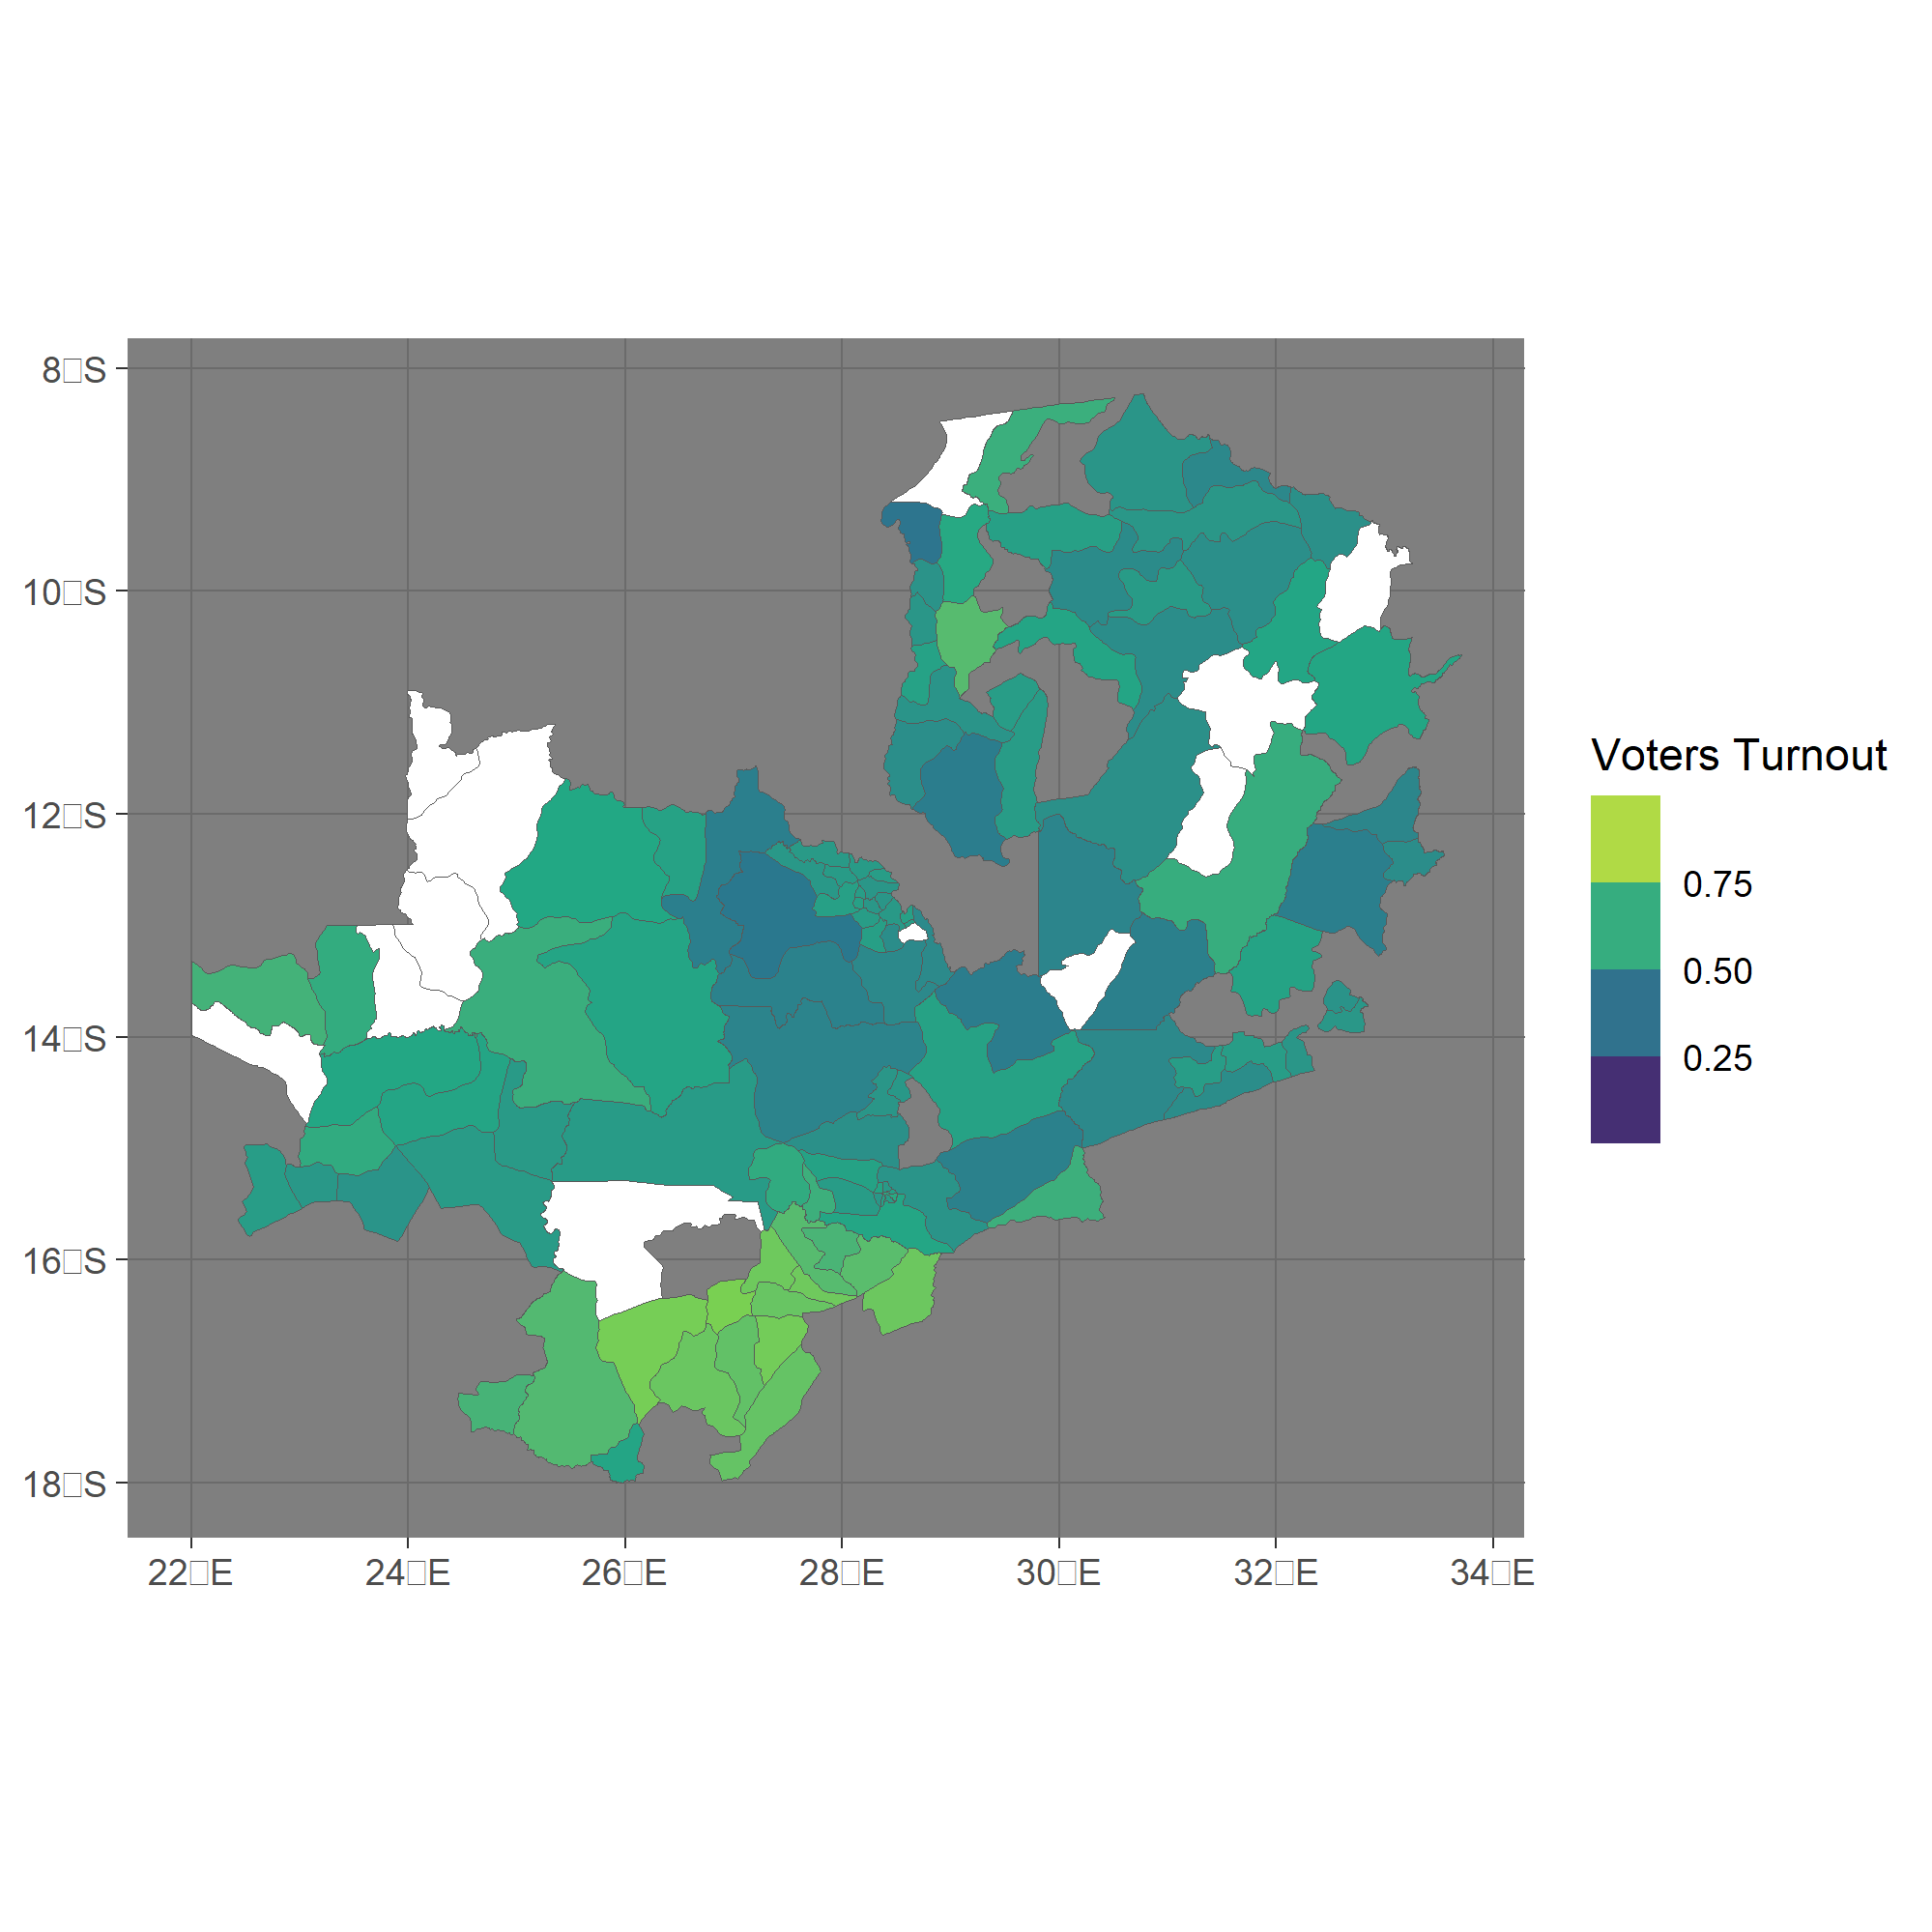
\includegraphics[width=6.25in,height=5.20833in]{outcome1.png}

It is already visible how the part of the country with a lower electoral
participation in in the center of the country, and remember that white
districts are those for which we have missing data.

\hypertarget{ii-number-of-votes-by-party}{%
\subsection{(II) Number of votes by
party}\label{ii-number-of-votes-by-party}}

To visualize this second outcome variable I first look at how the votes
shares are distributed in all the country and then I detail district by
district for the most important parties. Firstly we can see below a
histogram with the vote share by party by creating a dataset with only
party name and vote share and then plot it:

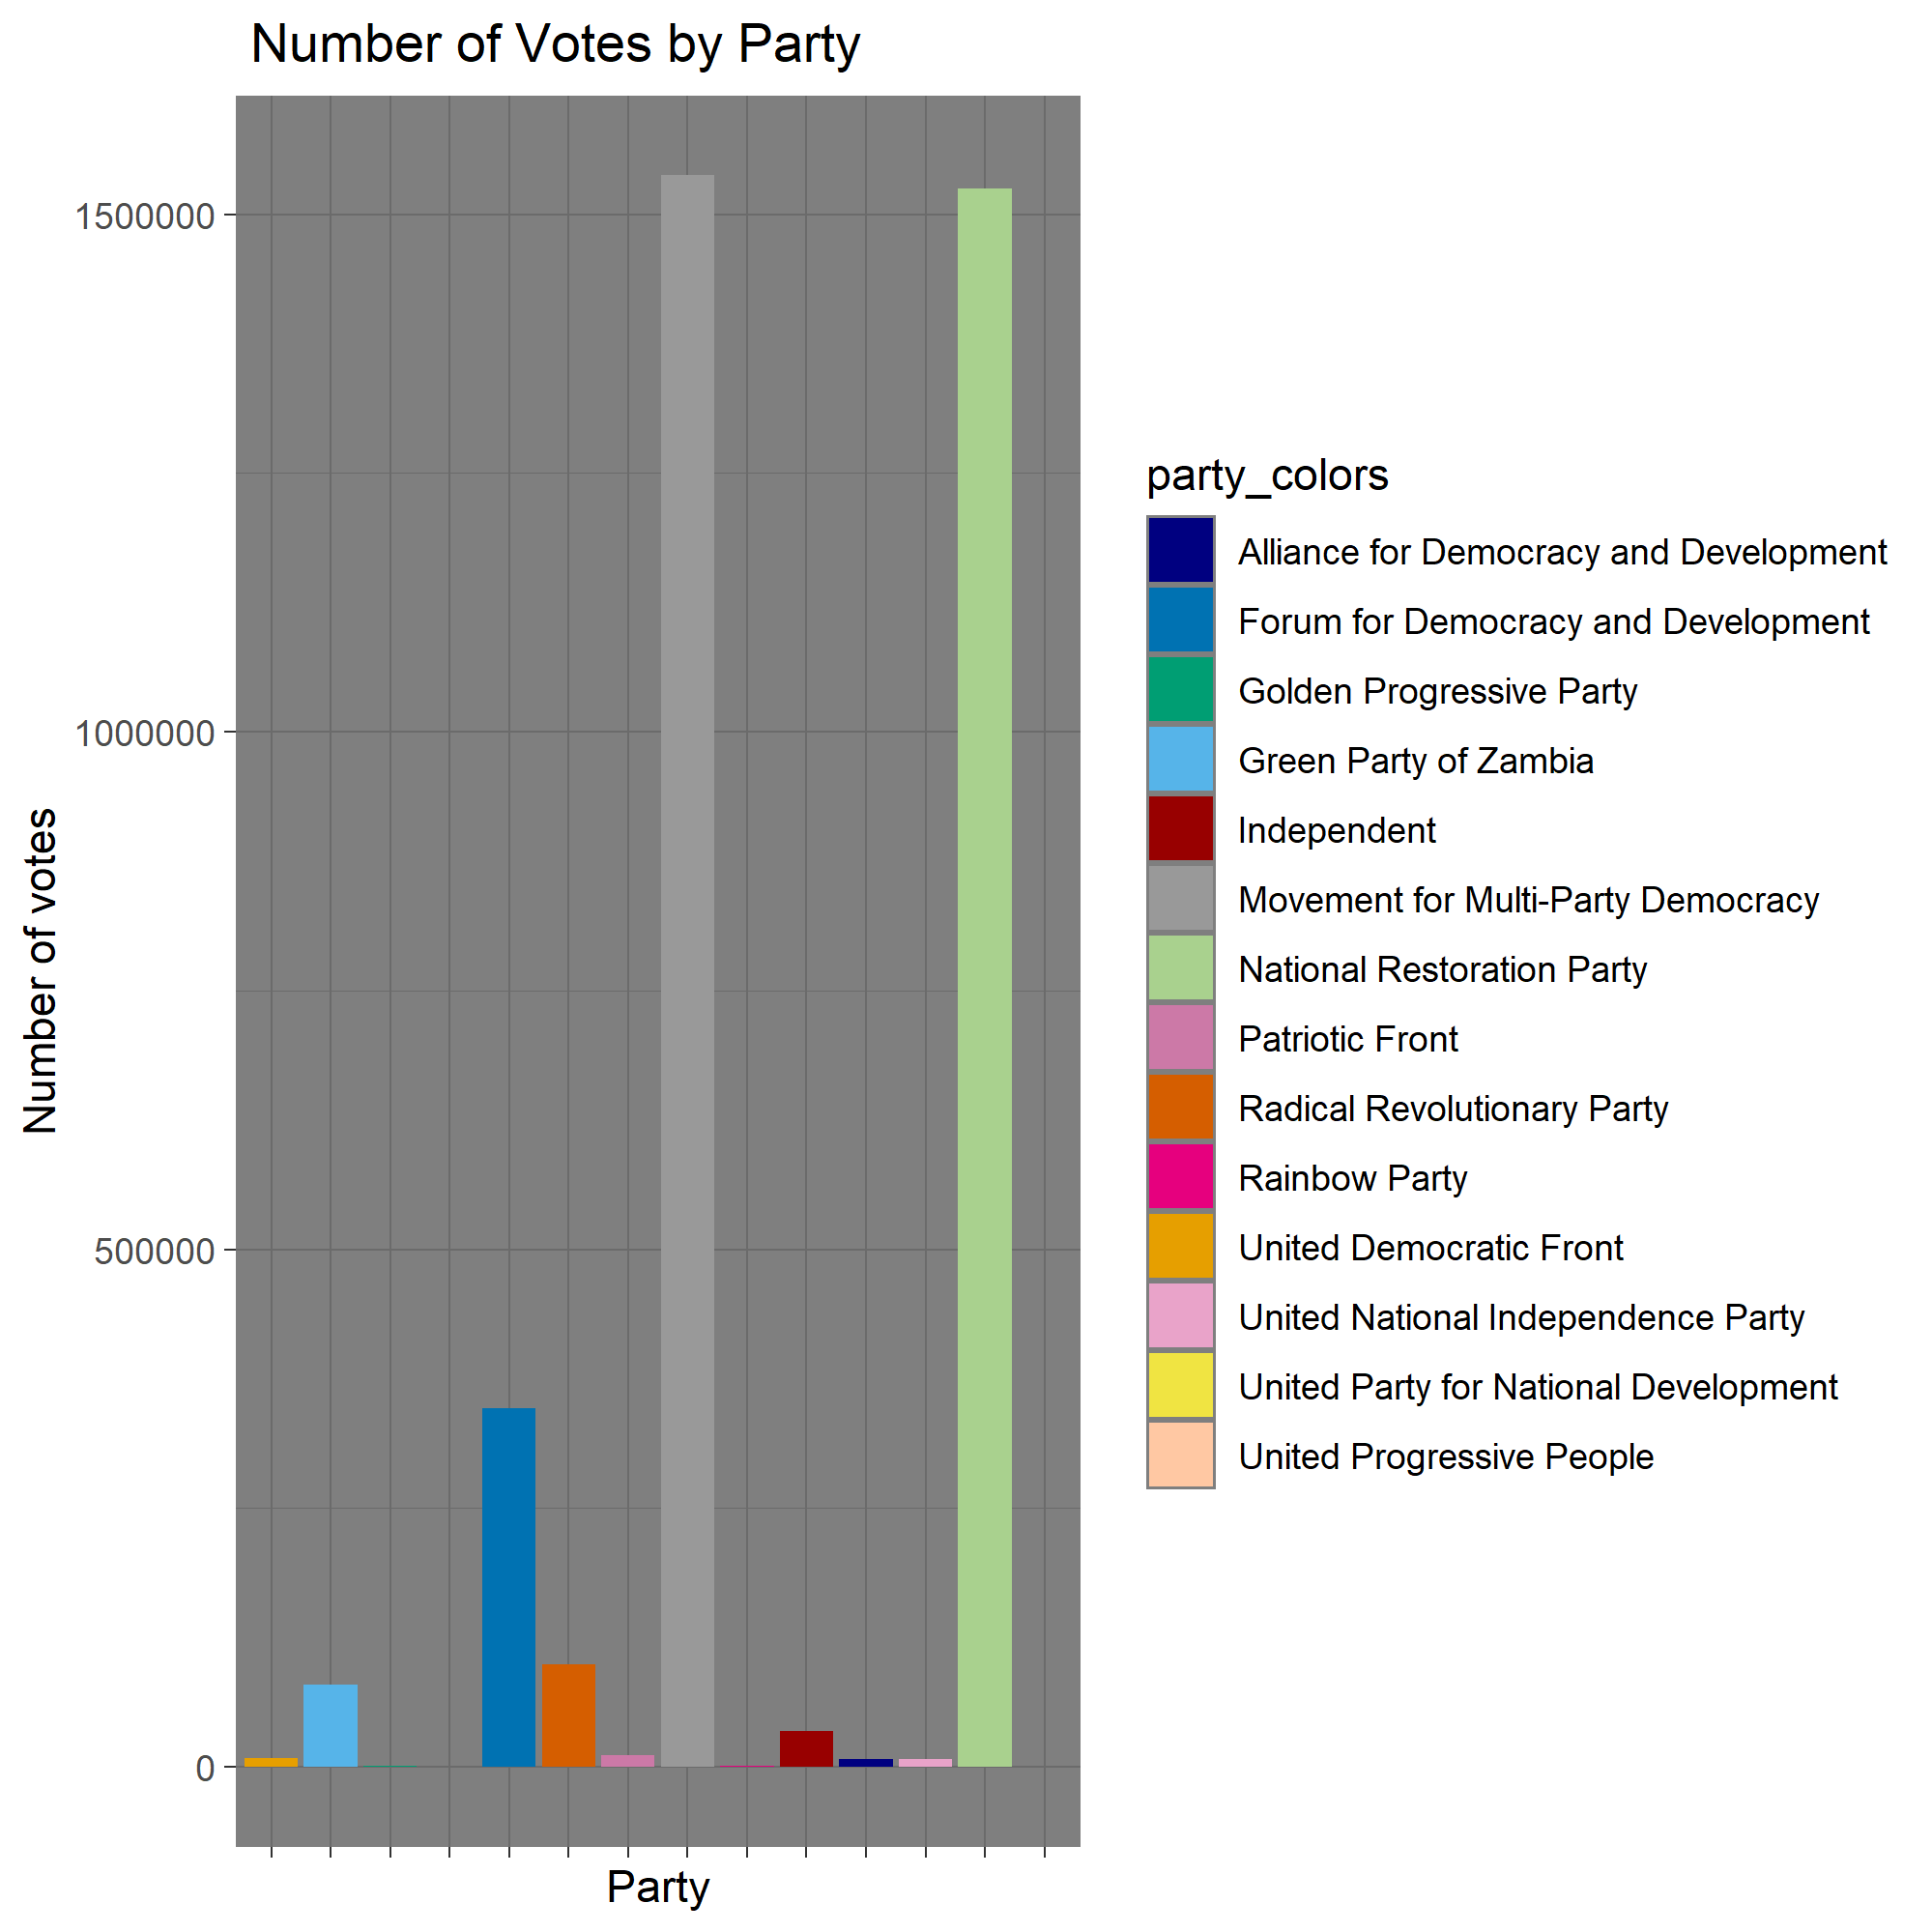
\includegraphics[width=8.33333in,height=5.20833in]{votesharebar.png}

The two main parties seem to be National Restoration Party and Movement
for Multi-Party Democracy.

Looking at how the votes for the two main parties are geographically
distributed :

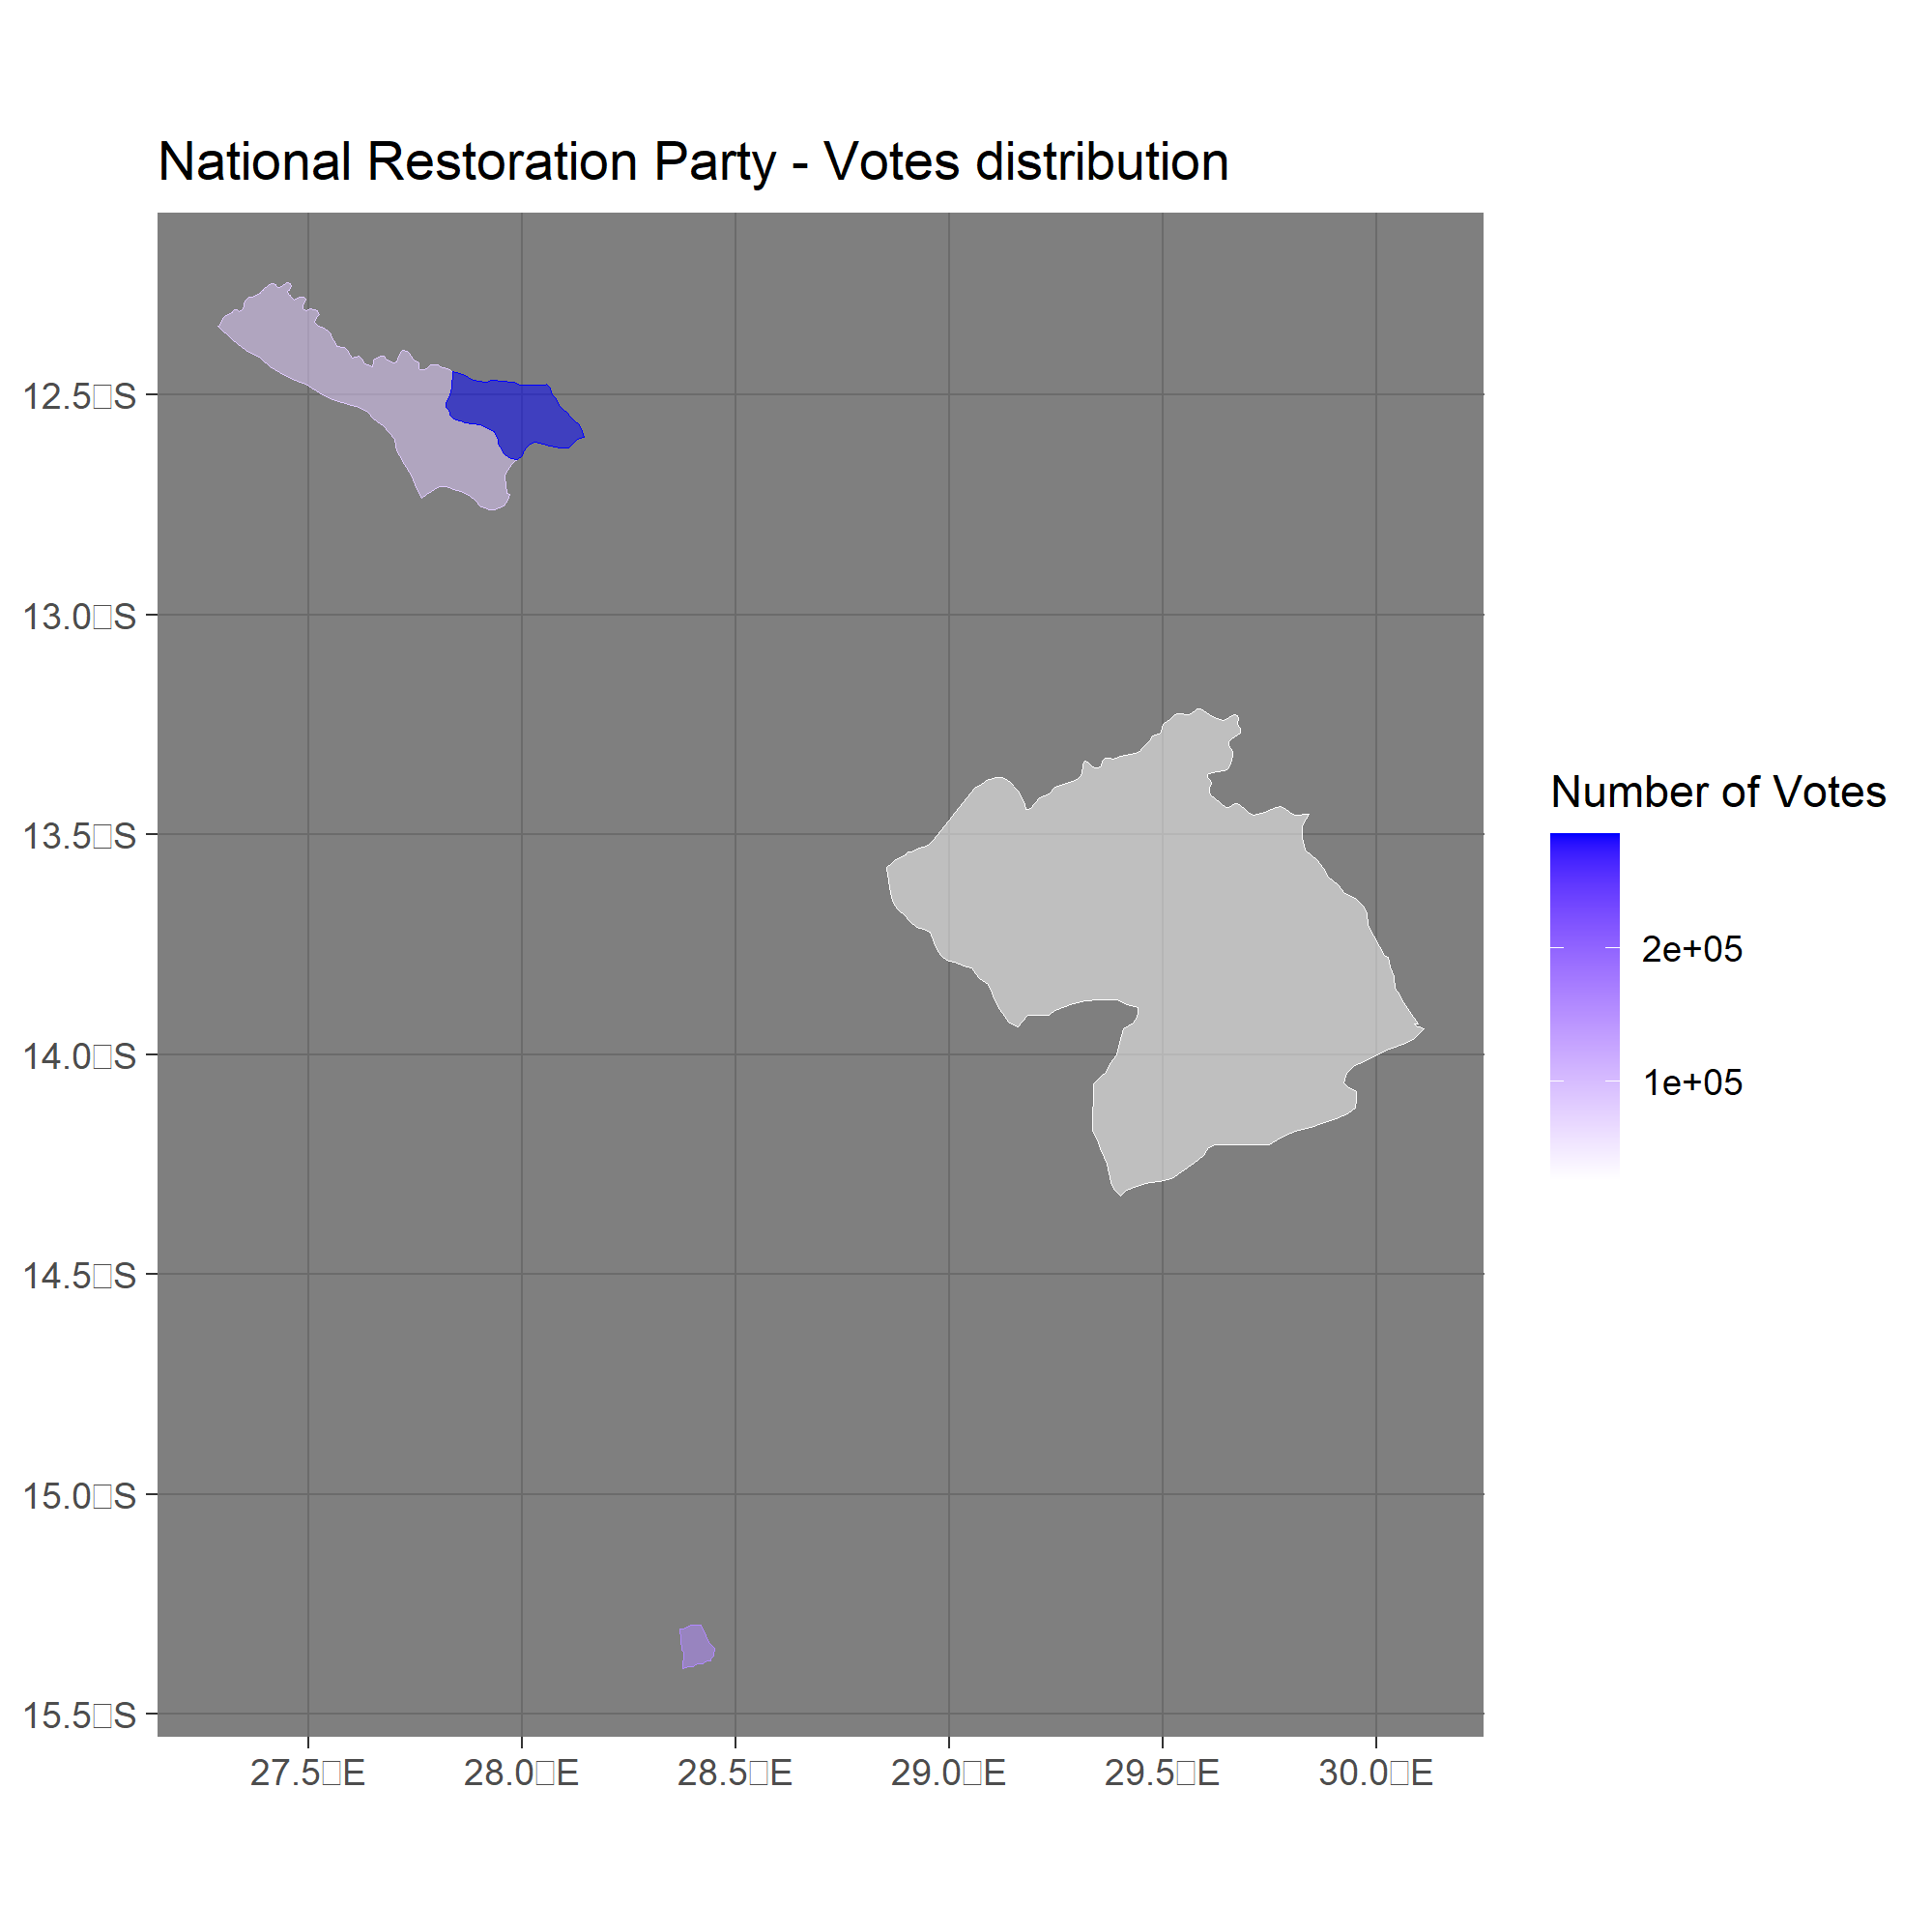
\includegraphics[width=5.20833in,height=4.16667in]{nrp.png}

NRP is receiving more votes in the north-east part of the country while
MPD is getting more support in the center where we could observe above
the turnout is higher and there is relatively more internet access

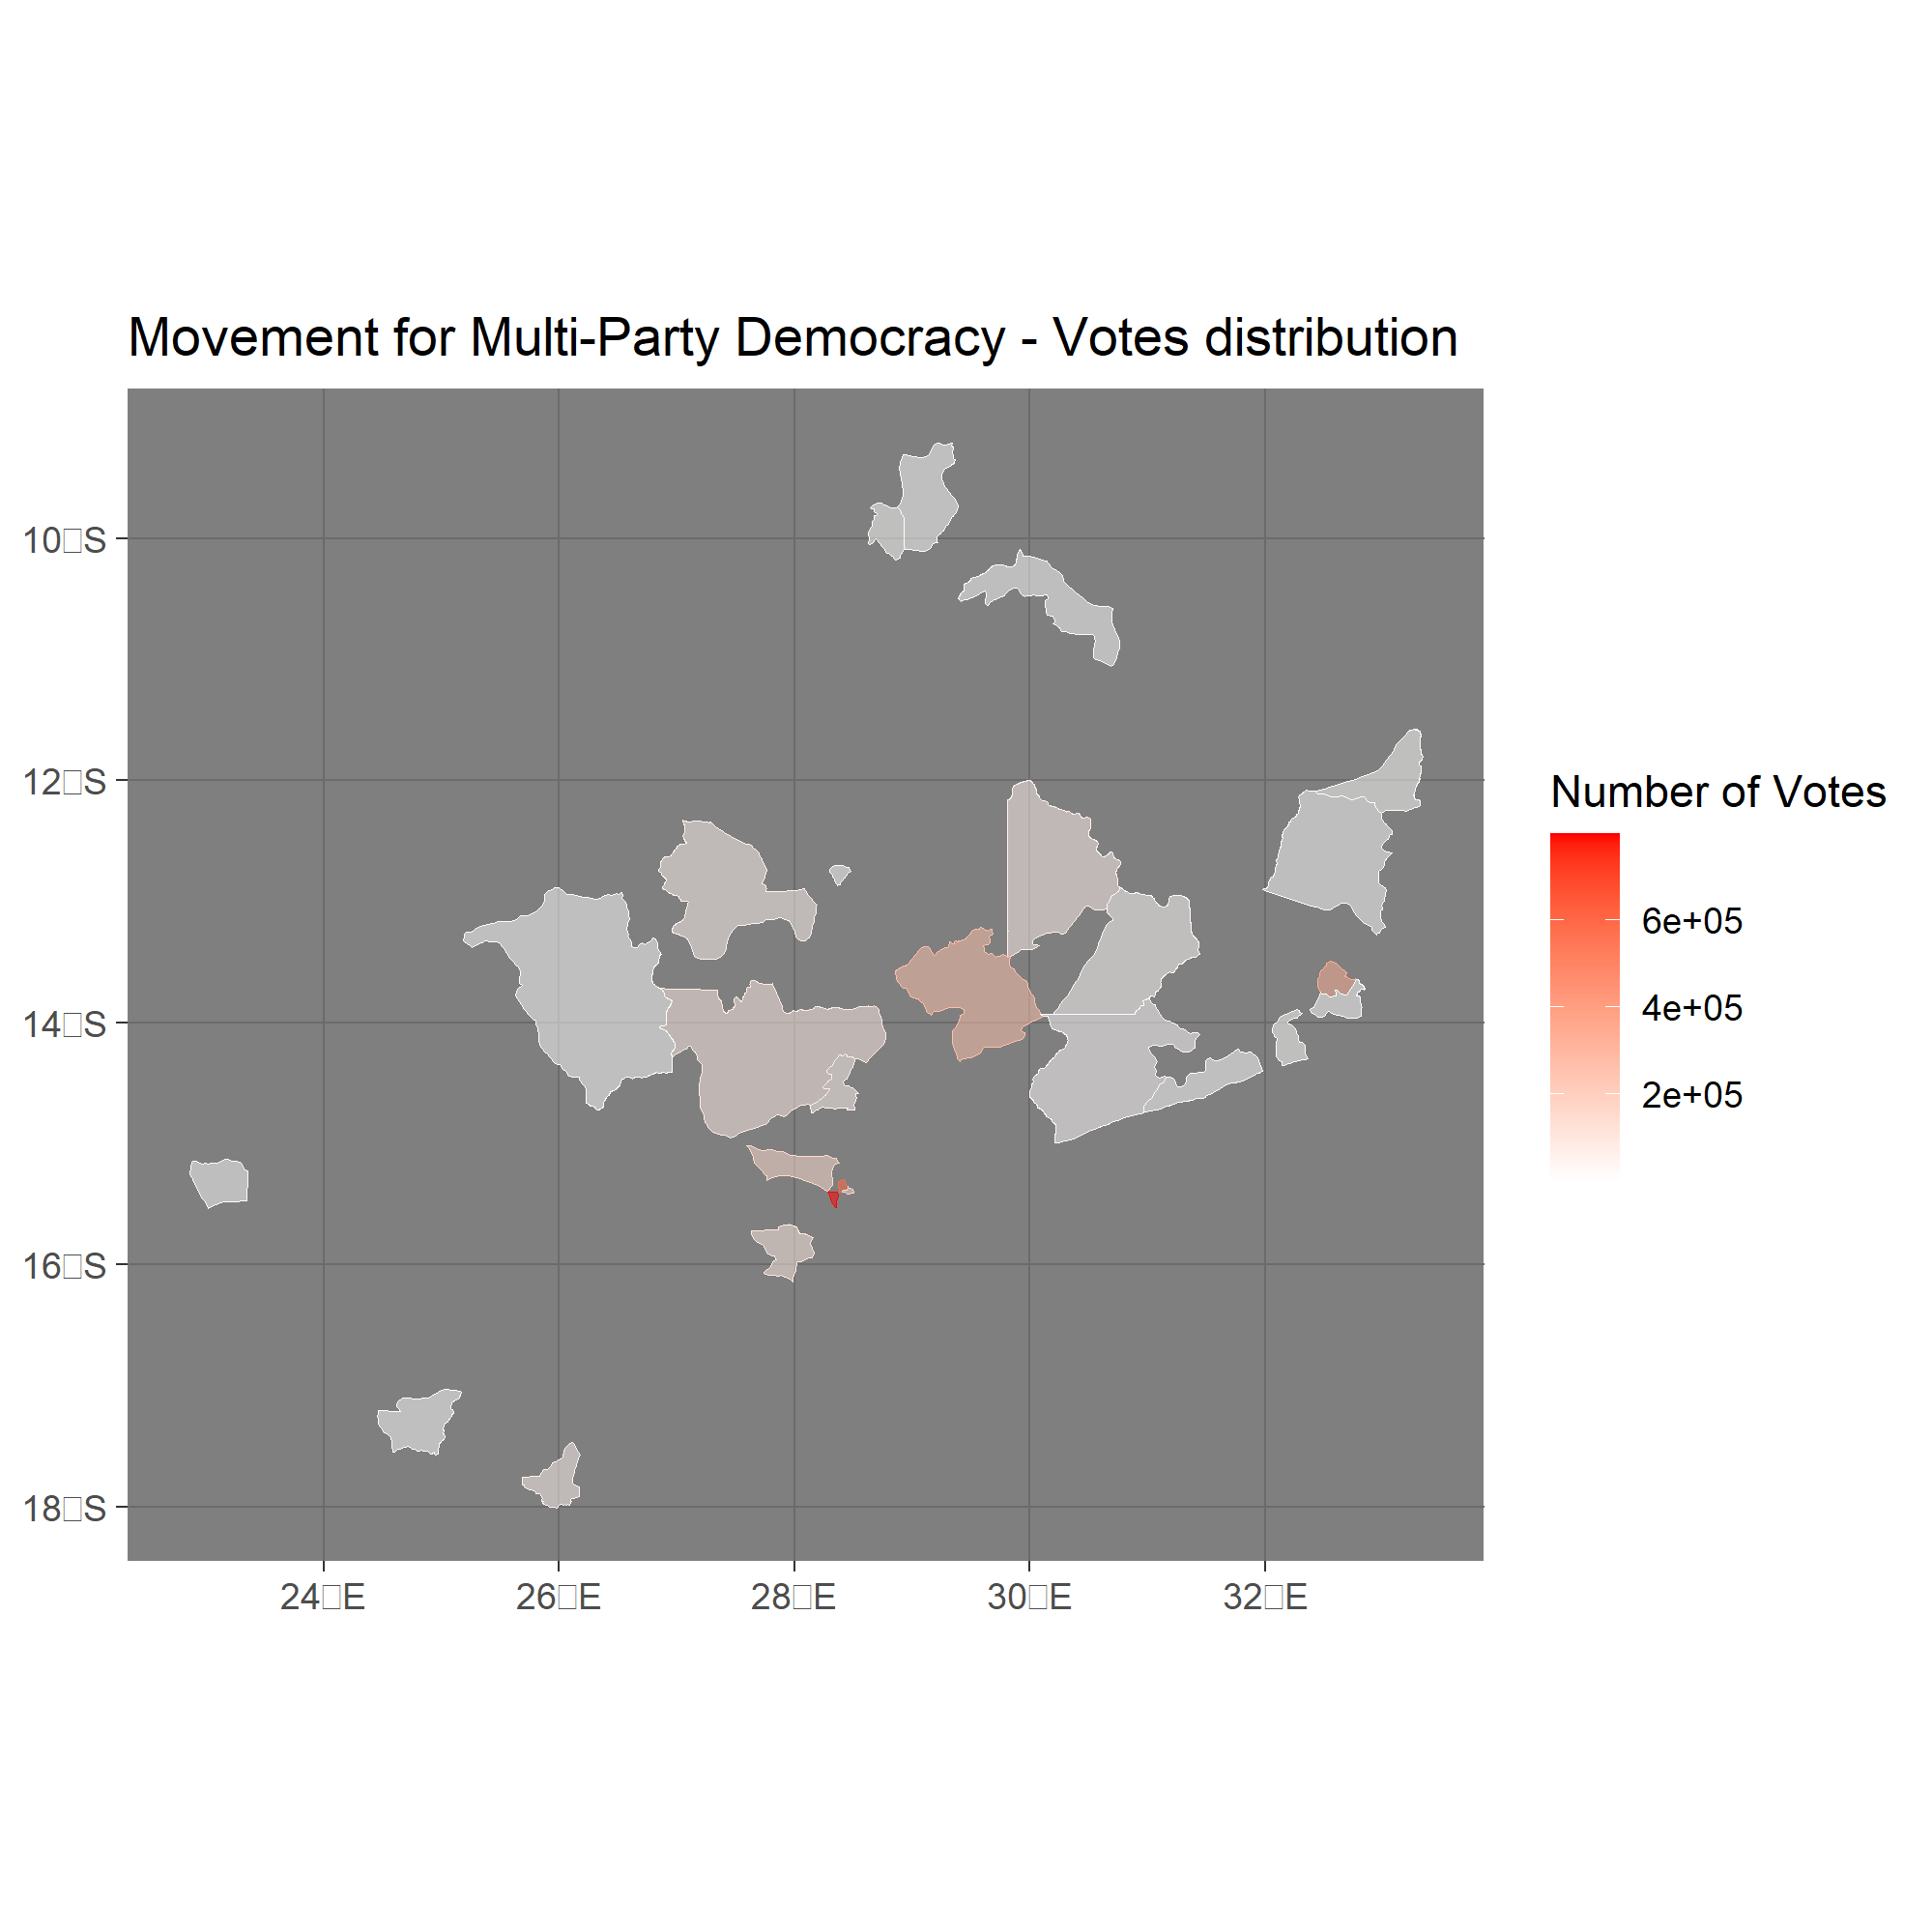
\includegraphics[width=5.20833in,height=4.16667in]{add.png}

Now I run the correlation between having at least one CID in your
district and the voters turnout using a maximum likelihood estimator and
I plot it filtering out NA:

\hypertarget{correlation-between-internet-access-and-voters-turnout}{%
\subsection{Correlation between internet access and voters'
turnout}\label{correlation-between-internet-access-and-voters-turnout}}

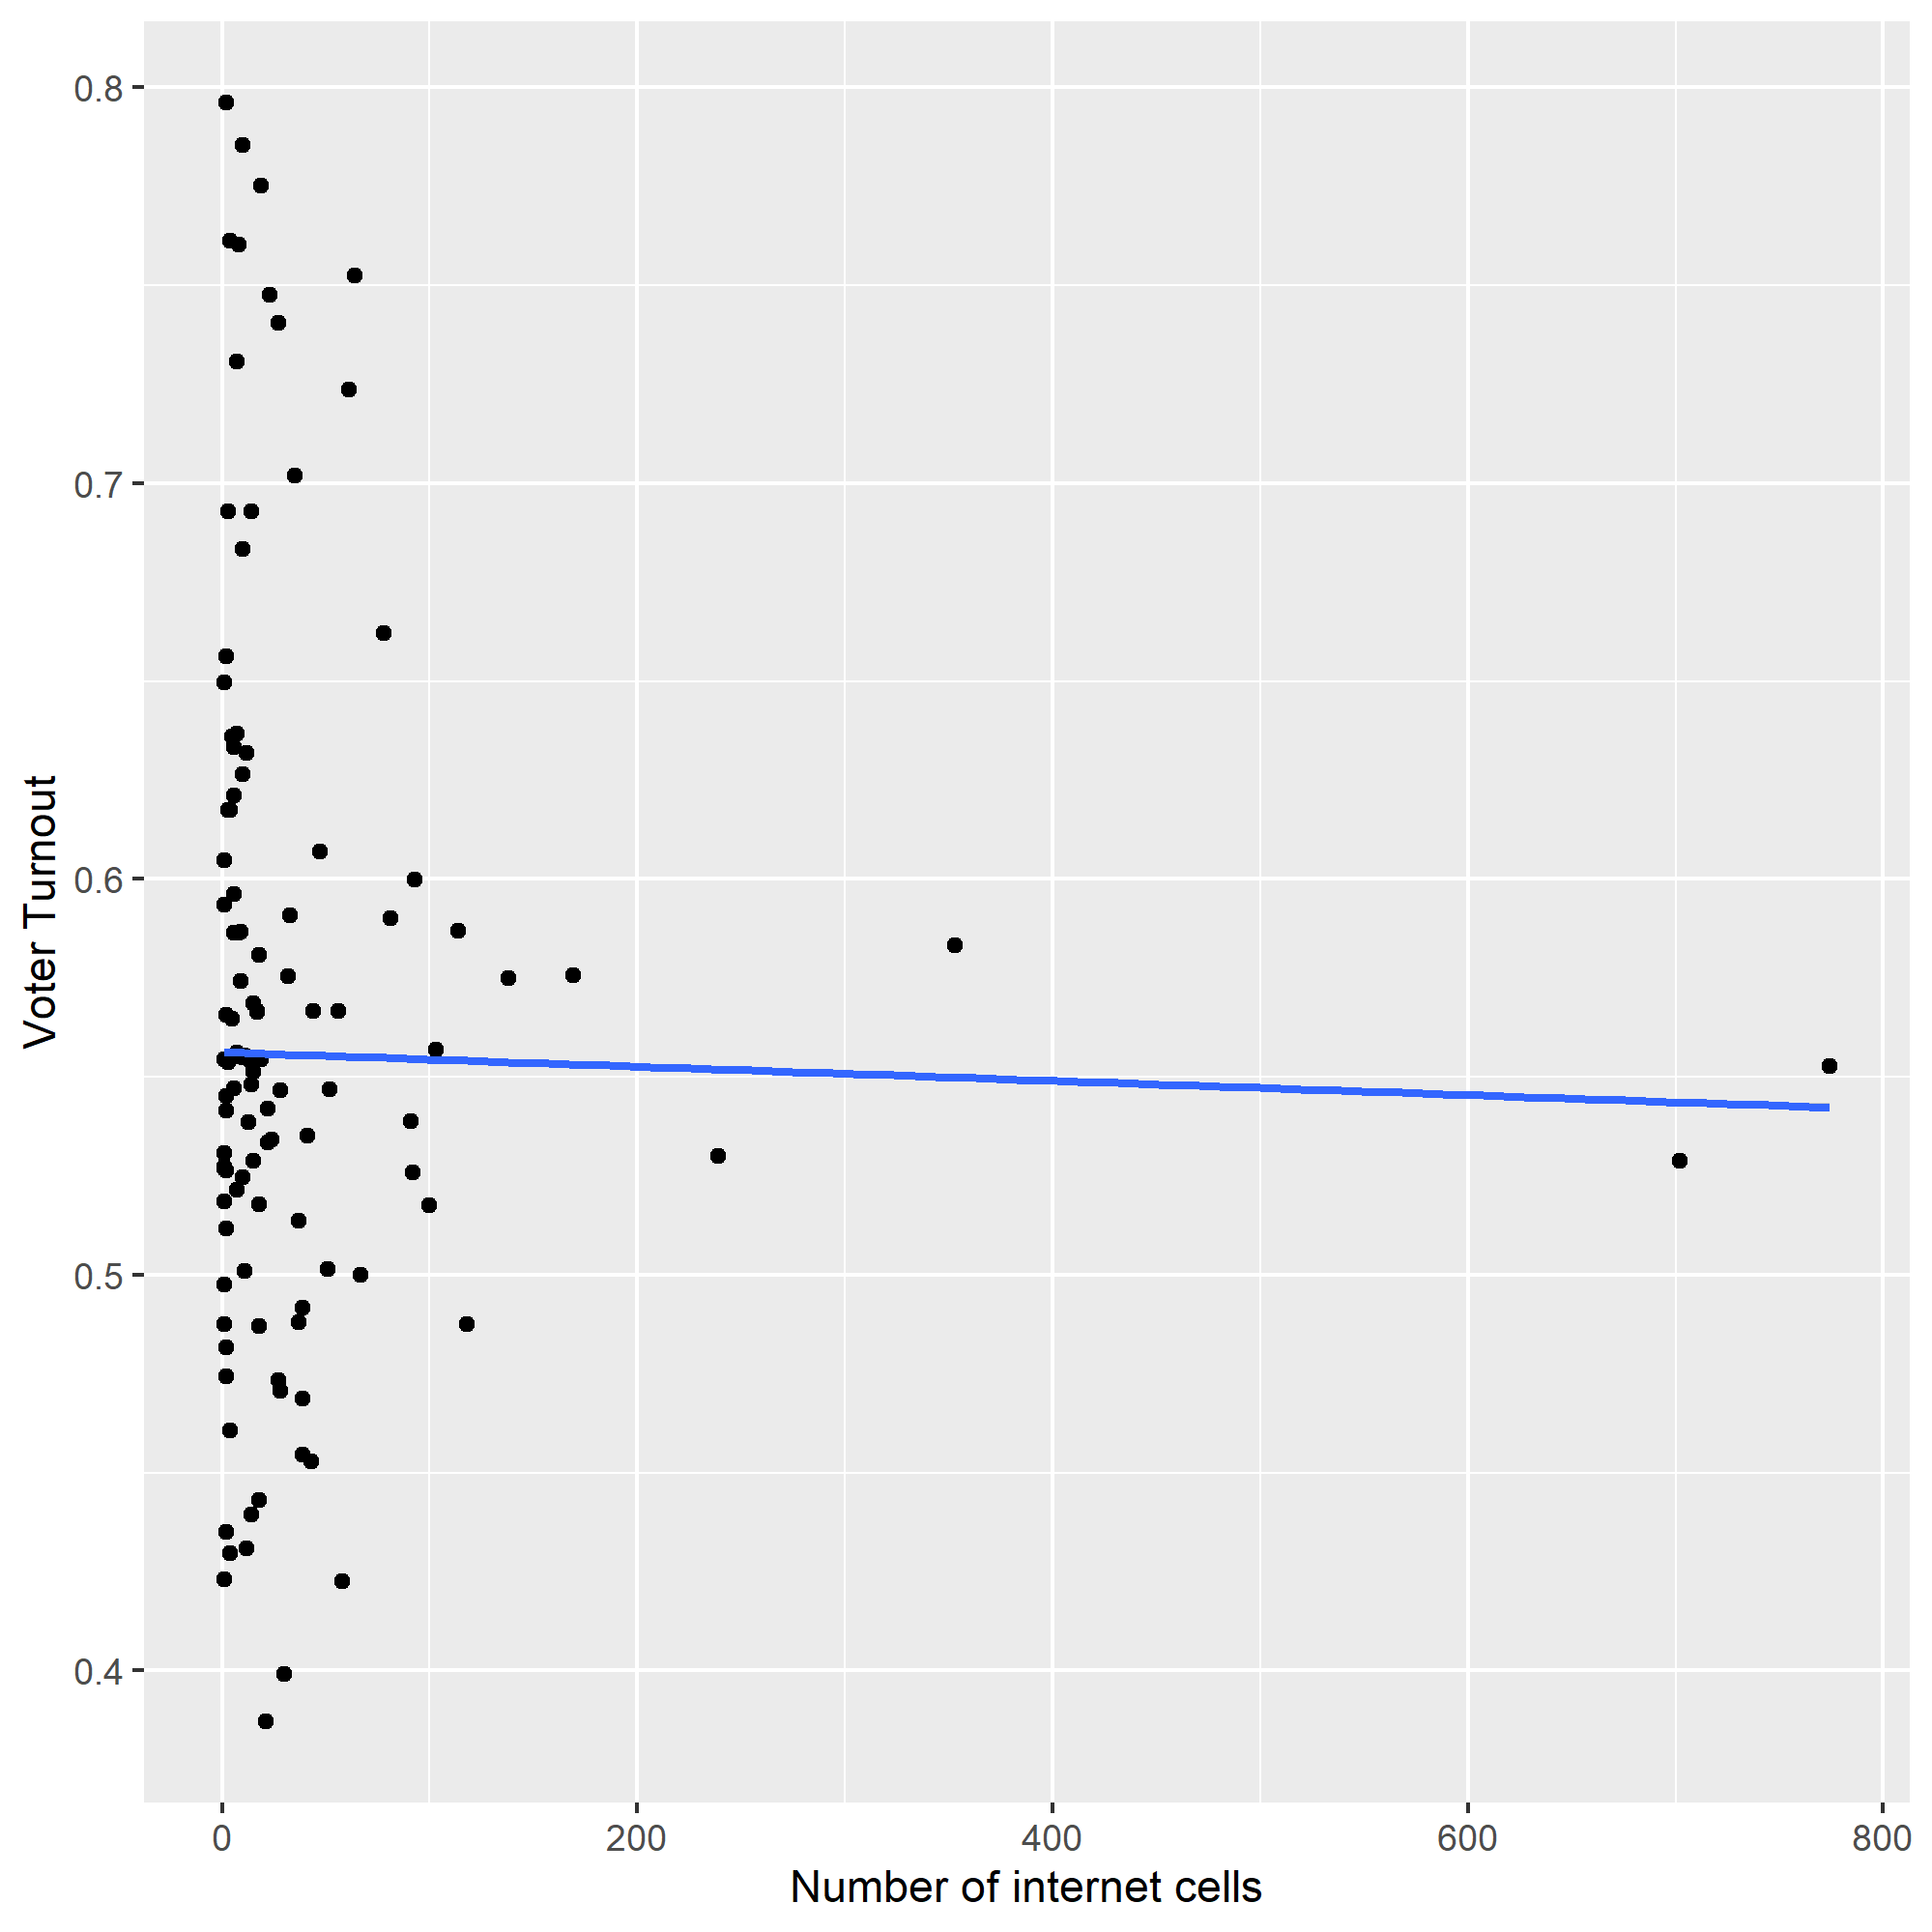
\includegraphics[width=6.25in,height=5.20833in]{lm.png}

It looks like there is no correlation between the intensity of the
treatment, internet access, and the voters turnout.

Now let's look at the correlation with the number of valid votes, maybe
internet connection comes with more awareness on electoral competition
rules:

\hypertarget{correlation-between-internet-access-and-number-of-valid-votes}{%
\subsection{Correlation between internet access and number of valid
votes}\label{correlation-between-internet-access-and-number-of-valid-votes}}

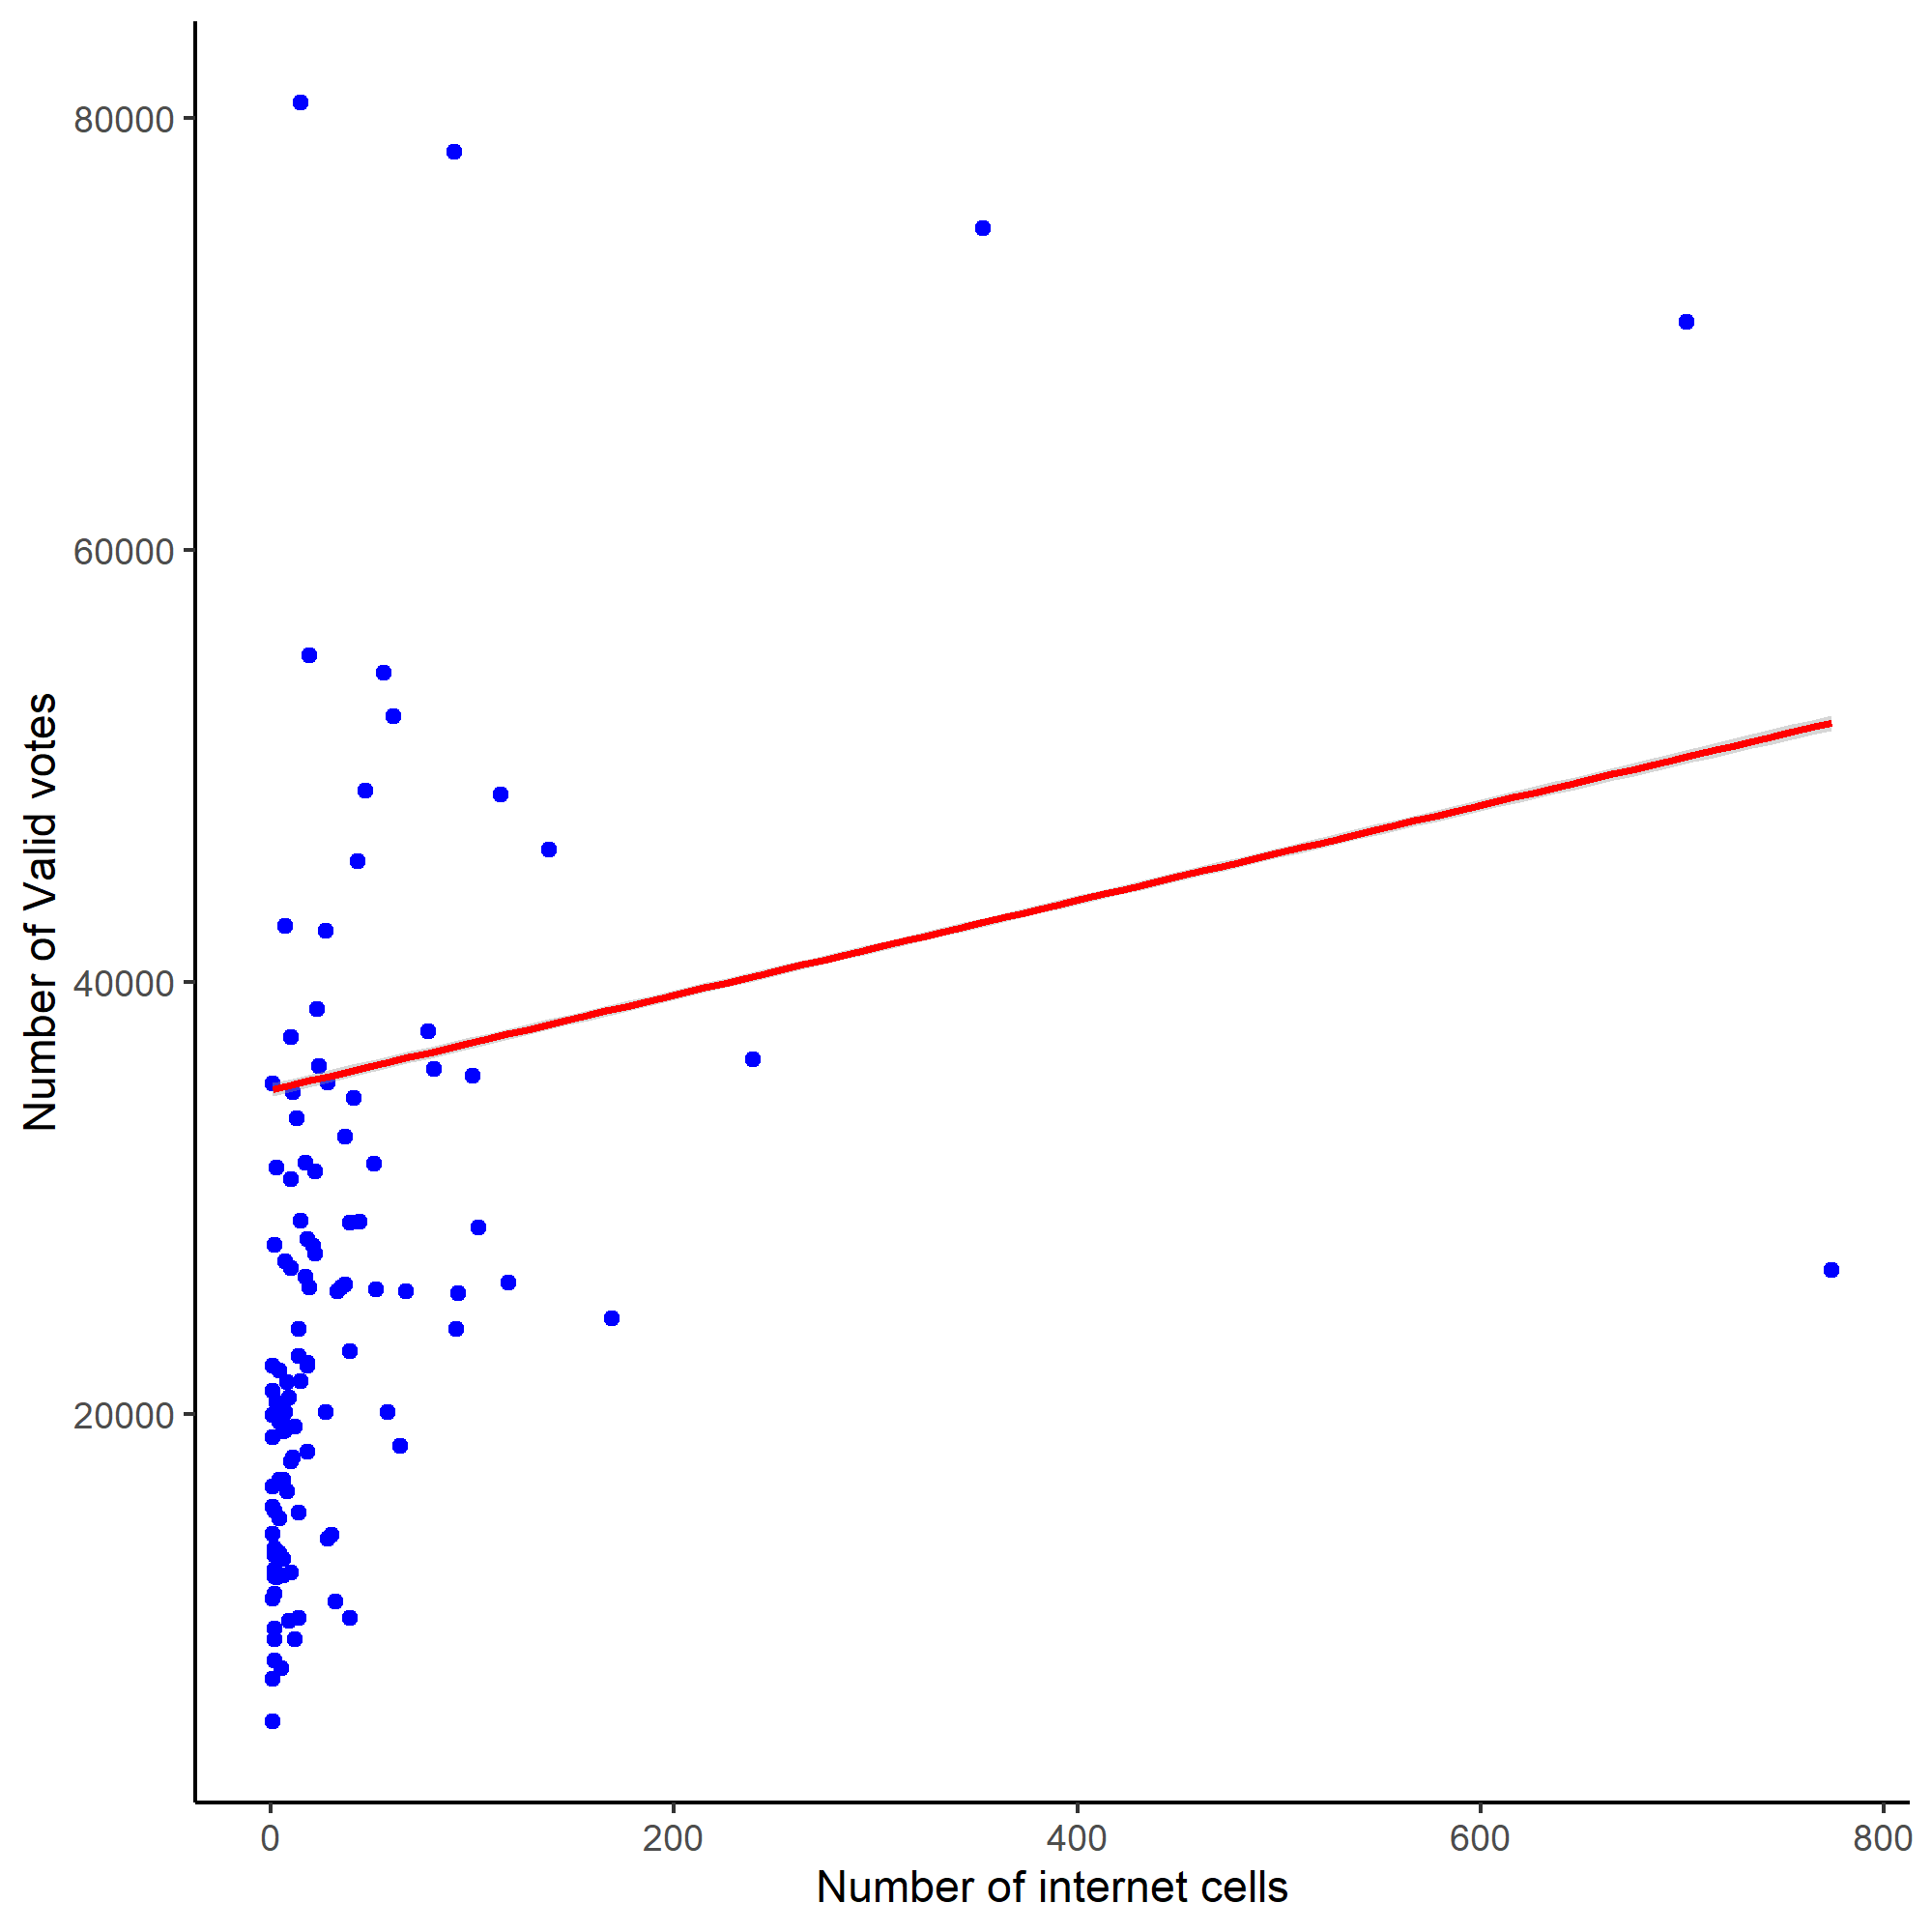
\includegraphics[width=6.25in,height=5.20833in]{comp.png}

The picture here looks very similar, little to no correlation is shown.

\hypertarget{second-treatment-assignment}{%
\subsubsection{Second Treatment
Assignment}\label{second-treatment-assignment}}

I can now assign the presence of internet access using the presence of
treatment instead of the intensity of the treatment and see if the lack
fo correlation is robust to this alternative treatment specification. To
do this I create a dummy that is 1 if there is at least 1 CID in the
electoral district and 0 otherwise adn then I plot it's distribution to
see if there is heterogeneity in how this new way of assigning treatment
look like.

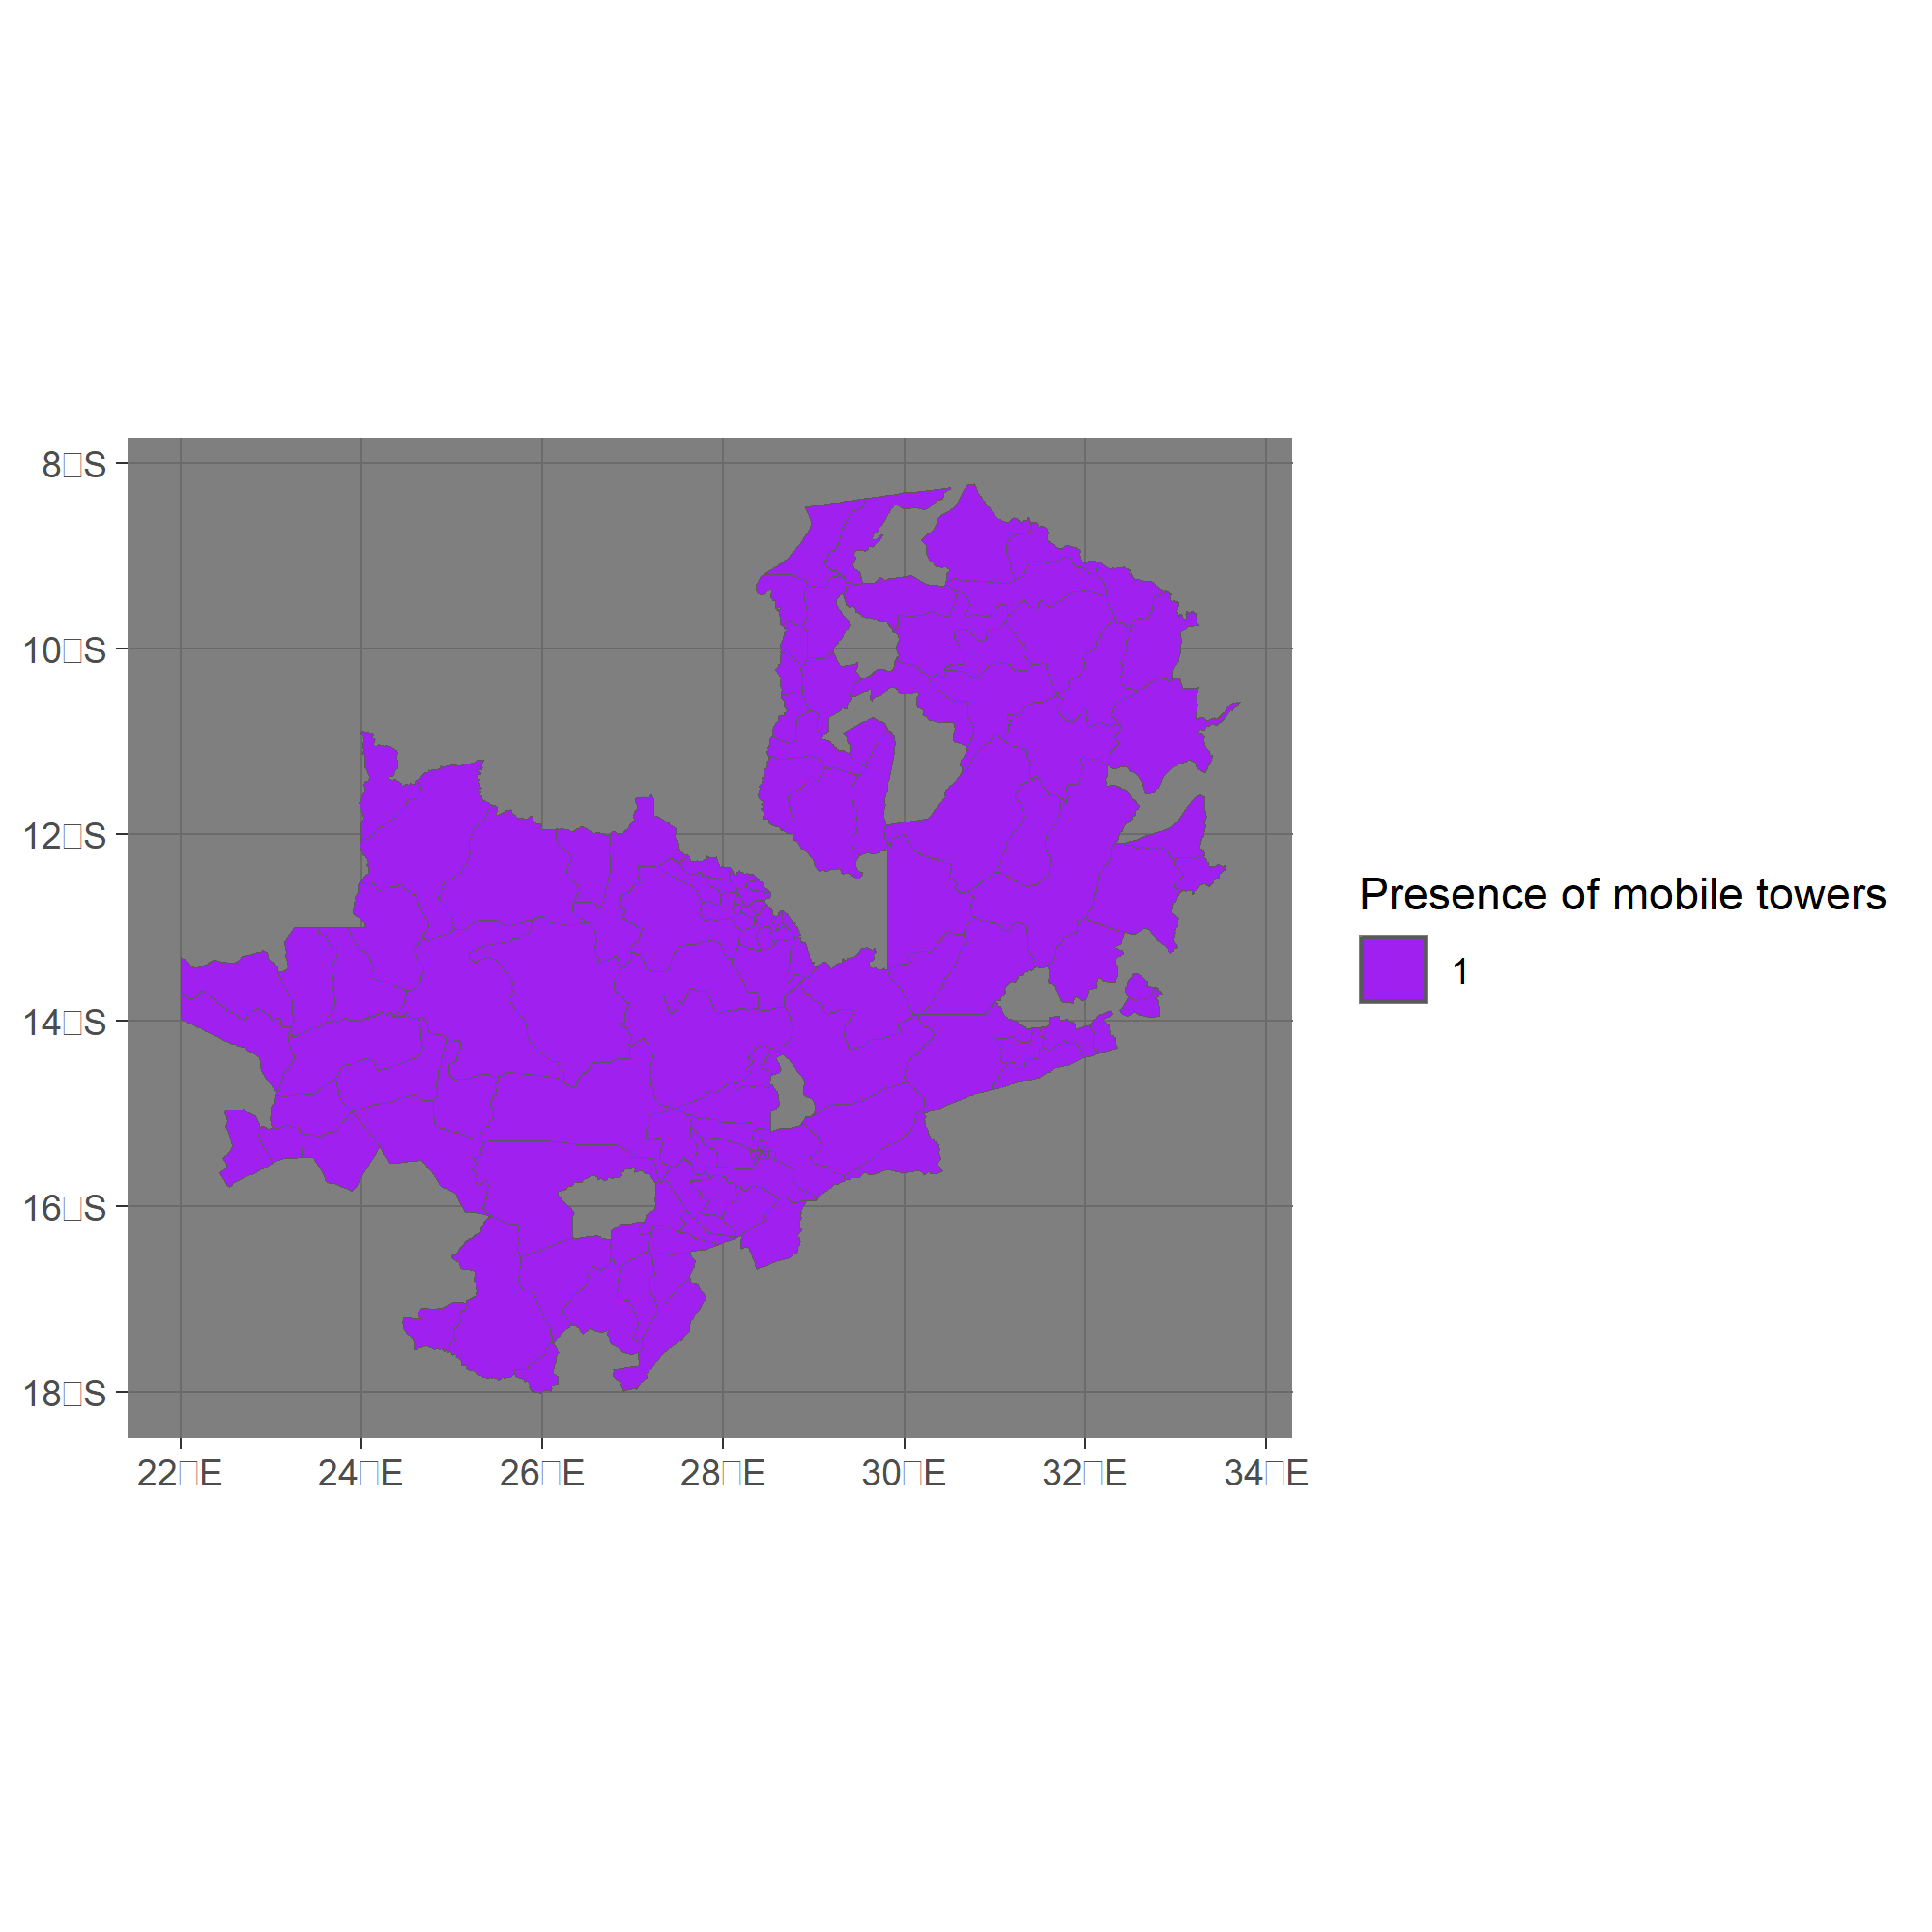
\includegraphics[width=6.25in,height=5.20833in]{treat2.png}

It is visible how in each district by 2016 there is still at least one
mobile tower registered, so this way of assigning treatment is not
useful for the purpose of the analysis.

\hypertarget{conclusion}{%
\section{Conclusion}\label{conclusion}}

In conclusion there is a lot of heterogeneity in terms of geographical
location for both the turnout, the party vote share, the number od
eligible votes and the presence of internet access mobile towers, but
the patterns do not seem to be correlated after this first exploration.

\hypertarget{explained-chunk-of-code}{%
\section{Explained chunk of code}\label{explained-chunk-of-code}}

I choose to explain in detail this chunk of code :

\begin{Shaded}
\begin{Highlighting}[]
\NormalTok{vote\_share }\OtherTok{\textless{}{-}}\NormalTok{ election\_2016 }\SpecialCharTok{|\textgreater{}}
  \FunctionTok{group\_by}\NormalTok{(party\_name) }\SpecialCharTok{|\textgreater{}}
  \FunctionTok{summarize}\NormalTok{(}\AttributeTok{total\_votes =} \FunctionTok{sum}\NormalTok{(n\_votes, }\AttributeTok{na.rm =} \ConstantTok{TRUE}\NormalTok{))}
\NormalTok{party\_colors }\OtherTok{\textless{}{-}} \FunctionTok{c}\NormalTok{(}\StringTok{"\#E69F00"}\NormalTok{, }\StringTok{"\#56B4E9"}\NormalTok{, }\StringTok{"\#009E73"}\NormalTok{, }\StringTok{"\#F0E442"}\NormalTok{,}
                           \StringTok{"\#0072B2"}\NormalTok{, }\StringTok{"\#D55E00"}\NormalTok{, }\StringTok{"\#CC79A7"}\NormalTok{,}
                           \StringTok{"\#999999"}\NormalTok{, }\StringTok{"\#E6007E"}\NormalTok{, }\StringTok{"\#980000"}\NormalTok{,}
                           \StringTok{"\#000080"}\NormalTok{, }\StringTok{"\#E9A3C9"}\NormalTok{, }\StringTok{"\#A9D18E"}\NormalTok{, }
                           \StringTok{"\#FFC8A3"}\NormalTok{)}
\FunctionTok{ggplot}\NormalTok{(vote\_share, }\FunctionTok{aes}\NormalTok{(}\AttributeTok{x =}\NormalTok{ party\_name, }\AttributeTok{y =}\NormalTok{ total\_votes, }\AttributeTok{fill =}\NormalTok{ party\_name)) }\SpecialCharTok{+} 
  \FunctionTok{geom\_bar}\NormalTok{(}\AttributeTok{stat =} \StringTok{"identity"}\NormalTok{) }\SpecialCharTok{+}
  \FunctionTok{labs}\NormalTok{(}\AttributeTok{title =} \StringTok{" Number of Votes by Party"}\NormalTok{, }\AttributeTok{x =} \StringTok{"Party"}\NormalTok{, }\AttributeTok{y =} \StringTok{"Number of votes"}\NormalTok{) }\SpecialCharTok{+}
  \FunctionTok{scale\_fill\_identity}\NormalTok{(}\AttributeTok{guide =} \StringTok{"legend"}\NormalTok{, }\AttributeTok{labels =}\NormalTok{ vote\_share}\SpecialCharTok{$}\NormalTok{party\_name) }\SpecialCharTok{+}
  \FunctionTok{theme\_dark}\NormalTok{() }\SpecialCharTok{+}
  \FunctionTok{theme}\NormalTok{(}\AttributeTok{axis.text.x =} \FunctionTok{element\_blank}\NormalTok{())}
\end{Highlighting}
\end{Shaded}

\hypertarget{section-2}{%
\subsubsection{1}\label{section-2}}

I create a subset of the election 2016 data where I have the sum of the
number of votes by party, to do this i group the n\_votes based on the
party name using the election\_2016 data and I aggregate by summing up
the n\_votes.

\hypertarget{section-3}{%
\subsubsection{2}\label{section-3}}

I create a list of colors, one for each party that I have in the
election data generating manually color scale.

\hypertarget{section-4}{%
\subsubsection{3}\label{section-4}}

I use ggplot setting the filtered votes by party as data, explaining in
the aesthetic that I want the x axis to be filled with the party names,
the y axis with how many votes and the fill should be based on the color
scale i created manually above.

\hypertarget{section-5}{%
\subsubsection{4}\label{section-5}}

The stat = ``identity'' argument tells ggplot that the y variable is
already in the correct scale and should be used as it is.

\hypertarget{section-6}{%
\subsubsection{5}\label{section-6}}

I use scale\_fill\_identity to produce a legend with the name of the
party and the assigned color at the side of the graph.

\hypertarget{section-7}{%
\subsubsection{6}\label{section-7}}

Lastly I set the theme to be dark because I like the style and I set off
the names of the parties in the x axis that was too crowded.

\end{document}
